\documentclass{article}

% Idioma y codificación
\usepackage[spanish, es-tabla]{babel}       %es-tabla para que se titule "Tabla"
\usepackage[utf8]{inputenc}

% Márgenes
\usepackage[a4paper,top=3cm,bottom=2.5cm,left=3cm,right=3cm]{geometry}

% Comentarios de bloque
\usepackage{verbatim}

% Paquetes de links
\usepackage[hidelinks]{hyperref}    % Permite enlaces
\usepackage{url}                    % redirecciona a la web

% Más opciones para enumeraciones
\usepackage{enumitem}

% Personalizar la portada
\usepackage{titling}


% Paquetes de tablas
\usepackage{multirow}


%------------------------------------------------------------------------

%Paquetes de figuras
\usepackage{caption}
\usepackage{subcaption} % Figuras al lado de otras
\usepackage{float}      % Poner figuras en el sitio indicado H.


% Paquetes de imágenes
\usepackage{graphicx}       % Paquete para añadir imágenes
\usepackage{transparent}    % Para manejar la opacidad de las figuras

% Paquete para usar colores
\usepackage[dvipsnames]{xcolor}
\usepackage{pagecolor}      % Para cambiar el color de la página

% Habilita tamaños de fuente mayores
\usepackage{fix-cm}


%------------------------------------------------------------------------

% Paquetes de matemáticas
\usepackage{mathtools, amsfonts, amssymb, mathrsfs}
\usepackage[makeroom]{cancel}     % Simplificar tachando
\usepackage{polynom}    % Divisiones y Ruffini
\usepackage{units} % Para poner fracciones diagonales con \nicefrac

\usepackage{pgfplots}   %Representar funciones
\pgfplotsset{compat=1.18}  % Versión 1.18

\usepackage{tikz-cd}    % Para usar diagramas de composiciones
\usetikzlibrary{calc}   % Para usar cálculo de coordenadas en tikz

%Definición de teoremas, etc.
\usepackage{amsthm}
%\swapnumbers   % Intercambia la posición del texto y de la numeración

\theoremstyle{plain}

\makeatletter
\@ifclassloaded{article}{
  \newtheorem{teo}{Teorema}[section]
}{
  \newtheorem{teo}{Teorema}[chapter]  % Se resetea en cada chapter
}
\makeatother

\newtheorem{coro}{Corolario}[teo]           % Se resetea en cada teorema
\newtheorem{prop}[teo]{Proposición}         % Usa el mismo contador que teorema
\newtheorem{lema}[teo]{Lema}                % Usa el mismo contador que teorema

\theoremstyle{remark}
\newtheorem*{observacion}{Observación}

\theoremstyle{definition}

\makeatletter
\@ifclassloaded{article}{
  \newtheorem{definicion}{Definición} [section]     % Se resetea en cada chapter
}{
  \newtheorem{definicion}{Definición} [chapter]     % Se resetea en cada chapter
}
\makeatother

\newtheorem*{notacion}{Notación}
\newtheorem*{ejemplo}{Ejemplo}
\newtheorem*{ejercicio*}{Ejercicio}             % No numerado
\newtheorem{ejercicio}{Ejercicio} [section]     % Se resetea en cada section


% Modificar el formato de la numeración del teorema "ejercicio"
\renewcommand{\theejercicio}{%
  \ifnum\value{section}=0 % Si no se ha iniciado ninguna sección
    \arabic{ejercicio}% Solo mostrar el número de ejercicio
  \else
    \thesection.\arabic{ejercicio}% Mostrar número de sección y número de ejercicio
  \fi
}


% \renewcommand\qedsymbol{$\blacksquare$}         % Cambiar símbolo QED
%------------------------------------------------------------------------

% Paquetes para encabezados
\usepackage{fancyhdr}
\pagestyle{fancy}
\fancyhf{}

\newcommand{\helv}{ % Modificación tamaño de letra
\fontfamily{}\fontsize{12}{12}\selectfont}
\setlength{\headheight}{15pt} % Amplía el tamaño del índice


%\usepackage{lastpage}   % Referenciar última pag   \pageref{LastPage}
\fancyfoot[C]{\thepage}

%------------------------------------------------------------------------

% Conseguir que no ponga "Capítulo 1". Sino solo "1."
\makeatletter
\@ifclassloaded{book}{
  \renewcommand{\chaptermark}[1]{\markboth{\thechapter.\ #1}{}} % En el encabezado
    
  \renewcommand{\@makechapterhead}[1]{%
  \vspace*{50\p@}%
  {\parindent \z@ \raggedright \normalfont
    \ifnum \c@secnumdepth >\m@ne
      \huge\bfseries \thechapter.\hspace{1em}\ignorespaces
    \fi
    \interlinepenalty\@M
    \Huge \bfseries #1\par\nobreak
    \vskip 40\p@
  }}
}
\makeatother

%------------------------------------------------------------------------
% Paquetes de cógido
\usepackage{minted}
\renewcommand\listingscaption{Código fuente}

\usepackage{fancyvrb}
% Personaliza el tamaño de los números de línea
\renewcommand{\theFancyVerbLine}{\small\arabic{FancyVerbLine}}

% Estilo para C++
\newminted{cpp}{
    frame=lines,
    framesep=2mm,
    baselinestretch=1.2,
    linenos,
    escapeinside=||
}



\usepackage{listings} % Para incluir código desde un archivo

\renewcommand\lstlistingname{Código Fuente}
\renewcommand\lstlistlistingname{Índice de Códigos Fuente}

% Definir colores
\definecolor{vscodepurple}{rgb}{0.5,0,0.5}
\definecolor{vscodeblue}{rgb}{0,0,0.8}
\definecolor{vscodegreen}{rgb}{0,0.5,0}
\definecolor{vscodegray}{rgb}{0.5,0.5,0.5}
\definecolor{vscodebackground}{rgb}{0.97,0.97,0.97}
\definecolor{vscodelightgray}{rgb}{0.9,0.9,0.9}

% Configuración para el estilo de C similar a VSCode
\lstdefinestyle{vscode_C}{
  backgroundcolor=\color{vscodebackground},
  commentstyle=\color{vscodegreen},
  keywordstyle=\color{vscodeblue},
  numberstyle=\tiny\color{vscodegray},
  stringstyle=\color{vscodepurple},
  basicstyle=\scriptsize\ttfamily,
  breakatwhitespace=false,
  breaklines=true,
  captionpos=b,
  keepspaces=true,
  numbers=left,
  numbersep=5pt,
  showspaces=false,
  showstringspaces=false,
  showtabs=false,
  tabsize=2,
  frame=tb,
  framerule=0pt,
  aboveskip=10pt,
  belowskip=10pt,
  xleftmargin=10pt,
  xrightmargin=10pt,
  framexleftmargin=10pt,
  framexrightmargin=10pt,
  framesep=0pt,
  rulecolor=\color{vscodelightgray},
  backgroundcolor=\color{vscodebackground},
}

%------------------------------------------------------------------------

% Comandos definidos
\newcommand{\bb}[1]{\mathbb{#1}}
\newcommand{\cc}[1]{\mathcal{#1}}

% I prefer the slanted \leq
\let\oldleq\leq % save them in case they're every wanted
\let\oldgeq\geq
\renewcommand{\leq}{\leqslant}
\renewcommand{\geq}{\geqslant}

% Si y solo si
\newcommand{\sii}{\iff}

% Letras griegas
\newcommand{\eps}{\epsilon}
\newcommand{\veps}{\varepsilon}
\newcommand{\lm}{\lambda}

\newcommand{\ol}{\overline}
\newcommand{\ul}{\underline}
\newcommand{\wt}{\widetilde}
\newcommand{\wh}{\widehat}

\let\oldvec\vec
\renewcommand{\vec}{\overrightarrow}

% Derivadas parciales
\newcommand{\del}[2]{\frac{\partial #1}{\partial #2}}
\newcommand{\Del}[3]{\frac{\partial^{#1} #2}{\partial^{#1} #3}}
\newcommand{\deld}[2]{\dfrac{\partial #1}{\partial #2}}
\newcommand{\Deld}[3]{\dfrac{\partial^{#1} #2}{\partial^{#1} #3}}


\newcommand{\AstIg}{\stackrel{(\ast)}{=}}
\newcommand{\Hop}{\stackrel{L'H\hat{o}pital}{=}}

\newcommand{\red}[1]{{\color{red}#1}} % Para integrales, destacar los cambios.

% Método de integración
\newcommand{\MetInt}[2]{
    \left[\begin{array}{c}
        #1 \\ #2
    \end{array}\right]
}

% Declarar aplicaciones
% 1. Nombre aplicación
% 2. Dominio
% 3. Codominio
% 4. Variable
% 5. Imagen de la variable
\newcommand{\Func}[5]{
    \begin{equation*}
        \begin{array}{rrll}
            #1:& #2 & \longrightarrow & #3\\
               & #4 & \longmapsto & #5
        \end{array}
    \end{equation*}
}

%------------------------------------------------------------------------

% Define a custom command for email addresses
\newcommand{\email}[1]{\href{mailto:#1}{{{\color{blue}#1}}}}


\usepackage{schemata}
\usepackage{ragged2e}
\usepackage{booktabs}

\definecolor{codegreen}{rgb}{0,0.6,0}
\definecolor{codegray}{rgb}{0.5,0.5,0.5}
\definecolor{codepurple}{rgb}{0.58,0,0.82}
\definecolor{backcolour}{rgb}{0.95,0.95,0.92}

\definecolor{backcolor}{RGB}{30,30,30}
\definecolor{codeblue}{RGB}{153,255,255}
\definecolor{codepink}{RGB}{200,80,180}
\definecolor{normalblue}{RGB}{12,144,244}

\lstdefinestyle{vscodestyle0}{
    backgroundcolor=\color{backcolor},   
    commentstyle=\color{codegreen},
    keywordstyle=\color{codepink},
    numberstyle=\tiny\color{codegray},
    identifierstyle=\color{codeblue},
    rulecolor=\color{black},
    stringstyle=\color{codepurple},
    basicstyle=\ttfamily\footnotesize,
    breakatwhitespace=false,         
    breaklines=true,                 
    captionpos=b,                    
    keepspaces=true,                 
    numbers=left,                    
    numbersep=5pt,                  
    showspaces=false,                
    showstringspaces=false,
    showtabs=false,                  
    tabsize=2,
    literate=%
  {\ +\ }{{{\color{Red}\ +\ }}}1
  {\ -\ }{{{\color{Red}\ -\ }}}1
  {\ *\ }{{{\color{Red}\ *\ }}}1
  {\ /\ }{{{\color{Red}\ /\ }}}1
  {\ =\ }{{{\color{Red}\ =\ }}}1
}

\lstdefinestyle{vscodestyle}{
    backgroundcolor=\color{backcolor},    % Fondo oscuro
    basicstyle=\color{white}\ttfamily\footnotesize, % Texto en blanco
    commentstyle=\color{green!50!black}, % Estilo de comentarios
    keywordstyle=\color{codepink},       % Estilo de palabras clave
    keywordstyle={[2]\color{blue}}, % Estilo para tipos de datos (int, char, double, etc.)
    identifierstyle=\color{codeblue},
    numberstyle=\tiny\color{gray},   % Estilo de números de línea
    stringstyle=\color{orange},      % Estilo de cadenas de texto
    rulecolor=\color{black},
    breakatwhitespace=false,         % Romper líneas solo en espacios en blanco
    breaklines=true,                 % Romper líneas automáticamente
    captionpos=b,                    % Posición de la leyenda (abajo)
    keepspaces=true,                 % Conservar espacios en blanco
    numbers=left,                    % Mostrar números de línea a la izquierda
    numbersep=5pt,                   % Separación de números de línea del código
    showspaces=false,                % Mostrar espacios con guiones bajos
    showstringspaces=false,          % No subrayar espacios en cadenas de texto
    showtabs=false,                  % No mostrar tabulaciones
    tabsize=4                        % Tamaño de la tabulación
}

\lstset{
    language=C++,
    morekeywords={int,char,ld,double}
}


\lstdefinestyle{mystyle}{
    backgroundcolor=\color{backcolour},   
    commentstyle=\color{codegreen},
    keywordstyle=\color{magenta},
    numberstyle=\tiny\color{codegray},
    stringstyle=\color{codepurple},
    %identifierstyle=\color{blue},
    basicstyle=\ttfamily\footnotesize,
    breakatwhitespace=false,         
    breaklines=true,                 
    captionpos=b,                    
    keepspaces=true,                 
    numbers=left,                    
    numbersep=5pt,                  
    showspaces=false,                
    showstringspaces=false,
    showtabs=false,                  
    tabsize=2
}
%\usemintedstyle[C++]{default}
\lstset{style=mystyle}

\newcommand{\myparagraph}[1]{\paragraph{#1}\mbox{}\\}
\newcommand\N{\ensuremath{\mathbb N}\space} 



\hypersetup{
    colorlinks=false, % Establece 'true' si quieres que el texto del enlace sea de color en lugar de tener un cuadro
    pdfborder={0 0 0}, % Establece el borde del enlace a 0 para eliminarlo
}


\begin{document}

    % 1. Foto de fondo
    % 2. Título
    % 3. Encabezado Izquierdo
    % 4. Color de fondo
    % 5. Coord x del titulo
    % 6. Coord y del titulo
    % 7. Fecha
    % 8. Autor

    
    % 1. Foto de fondo
% 2. Título
% 3. Encabezado Izquierdo
% 4. Color de fondo
% 5. Coord x del titulo
% 6. Coord y del titulo
% 7. Fecha

\newcommand{\portada}[7]{

    \portadaBase{#1}{#2}{#3}{#4}{#5}{#6}{#7}
    \portadaBook{#1}{#2}{#3}{#4}{#5}{#6}{#7}
}

\newcommand{\portadaExamen}[7]{

    \portadaBase{#1}{#2}{#3}{#4}{#5}{#6}{#7}
    \portadaArticle{#1}{#2}{#3}{#4}{#5}{#6}{#7}
}




\newcommand{\portadaBase}[7]{

    % Tiene la portada principal y la licencia Creative Commons
    
    % 1. Foto de fondo
    % 2. Título
    % 3. Encabezado Izquierdo
    % 4. Color de fondo
    % 5. Coord x del titulo
    % 6. Coord y del titulo
    % 7. Fecha
    
    
    \thispagestyle{empty}               % Sin encabezado ni pie de página
    \newgeometry{margin=0cm}        % Márgenes nulos para la primera página
    
    
    % Encabezado
    \fancyhead[L]{\helv #3}
    \fancyhead[R]{\helv \nouppercase{\leftmark}}
    
    
    \pagecolor{#4}        % Color de fondo para la portada
    
    \begin{figure}[p]
        \centering
        \transparent{0.3}           % Opacidad del 30% para la imagen
        
        \includegraphics[width=\paperwidth, keepaspectratio]{assets/#1}
    
        \begin{tikzpicture}[remember picture, overlay]
            \node[anchor=north west, text=white, opacity=1, font=\fontsize{60}{90}\selectfont\bfseries\sffamily, align=left] at (#5, #6) {#2};
            
            \node[anchor=south east, text=white, opacity=1, font=\fontsize{12}{18}\selectfont\sffamily, align=right] at (9.7, 3) {\textbf{\href{https://losdeldgiim.github.io/}{Los Del DGIIM}}};
            
            \node[anchor=south east, text=white, opacity=1, font=\fontsize{12}{15}\selectfont\sffamily, align=right] at (9.7, 1.8) {Doble Grado en Ingeniería Informática y Matemáticas\\Universidad de Granada};
        \end{tikzpicture}
    \end{figure}
    
    
    \restoregeometry        % Restaurar márgenes normales para las páginas subsiguientes
    \pagecolor{white}       % Restaurar el color de página
    
    
    \newpage
    \thispagestyle{empty}               % Sin encabezado ni pie de página
    \begin{tikzpicture}[remember picture, overlay]
        \node[anchor=south west, inner sep=3cm] at (current page.south west) {
            \begin{minipage}{0.5\paperwidth}
                \href{https://creativecommons.org/licenses/by-nc-nd/4.0/}{
                    
\includegraphics[height=2cm]{assets/Licencia.png}
                }\vspace{1cm}\\
                Esta obra está bajo una
                \href{https://creativecommons.org/licenses/by-nc-nd/4.0/}{
                    Licencia Creative Commons Atribución-NoComercial-SinDerivadas 4.0 Internacional (CC BY-NC-ND 4.0).
                }\\
    
                Eres libre de compartir y redistribuir el contenido de esta obra en cualquier medio o formato, siempre y cuando des el crédito adecuado a los autores originales y no persigas fines comerciales. 
            \end{minipage}
        };
    \end{tikzpicture}
    
    
    
    % 1. Foto de fondo
    % 2. Título
    % 3. Encabezado Izquierdo
    % 4. Color de fondo
    % 5. Coord x del titulo
    % 6. Coord y del titulo
    % 7. Fecha


}


\newcommand{\portadaBook}[7]{

    % 1. Foto de fondo
    % 2. Título
    % 3. Encabezado Izquierdo
    % 4. Color de fondo
    % 5. Coord x del titulo
    % 6. Coord y del titulo
    % 7. Fecha

    % Personaliza el formato del título
    \pretitle{\begin{center}\bfseries\fontsize{42}{56}\selectfont}
    \posttitle{\par\end{center}\vspace{2em}}
    
    % Personaliza el formato del autor
    \preauthor{\begin{center}\Large}
    \postauthor{\par\end{center}\vfill}
    
    % Personaliza el formato de la fecha
    \predate{\begin{center}\huge}
    \postdate{\par\end{center}\vspace{2em}}
    
    \title{#2}
    \author{\href{https://losdeldgiim.github.io/}{Los Del DGIIM}}
    \date{Granada, #7}
    \maketitle
    
    \tableofcontents
}




\newcommand{\portadaArticle}[7]{

    % 1. Foto de fondo
    % 2. Título
    % 3. Encabezado Izquierdo
    % 4. Color de fondo
    % 5. Coord x del titulo
    % 6. Coord y del titulo
    % 7. Fecha

    % Personaliza el formato del título
    \pretitle{\begin{center}\bfseries\fontsize{42}{56}\selectfont}
    \posttitle{\par\end{center}\vspace{2em}}
    
    % Personaliza el formato del autor
    \preauthor{\begin{center}\Large}
    \postauthor{\par\end{center}\vspace{3em}}
    
    % Personaliza el formato de la fecha
    \predate{\begin{center}\huge}
    \postdate{\par\end{center}\vspace{5em}}
    
    \title{#2}
    \author{\href{https://losdeldgiim.github.io/}{Los Del DGIIM}}
    \date{Granada, #7}
    \thispagestyle{empty}               % Sin encabezado ni pie de página
    \maketitle
    \vfill
}
    \portada{etsiitA4.jpg}{Algorítmica\\Práctica 4}{Algorítmica. Práctica 4. B\&B y BK.}{MidnightBlue}{-8}{28}{2023-2024}{Laura Mandow Fuentes\\Chengcheng Liu\\Daniel Hidalgo Chica\\Roberto González Lugo\\Elías Monge Sánchez}

    \newpage

    
\section{Participación}
    \begin{itemize}
        \item Laura Mandow Fuentes. \email{e.lauramandow@go.ugr.es}  $100\%$
        \item Roberto González Lugo. \email{e.roberlks222@go.ugr.es}  $100\%$
        \item Daniel Hidalgo Chica. \email{e.danielhc@go.ugr.es}  $100\%$
        \item Chengcheng Liu. \email{e.cliu04@go.ugr.es} $100\%$
        \item Elías Monge Sánchez. \email{e.eliasmonge234@go.ugr.es}  $100\%$
    \end{itemize}
    \subsection{Participación específica}
    Aunque hayamos trabajado cada uno de forma global los contenidos de la práctica, a la hora de la redacción de la memoria, el trabajo se ha visto dividido en partes de carga de trabajo similar con el fin de aumentar la productividad.
    \\
    En particular, las máquinas utilizadas para ejecutar los algoritmos son:

    \begin{itemize}
        \item Maquina 1
        \begin{itemize}
                \item Máquina: Asus TUF fx505dt
                \item Procesador: AMD Ryzen 7 3750h with Radeon Vega Mobile Gfx 2.3GHz
                \item Tarjeta gráfica: Nvidia Geforce GTX 1650
                \item Sistema Operativo: Arch Linux 64bits
        \end{itemize}

        \item Maquina 2
        \begin{itemize}

                \item Máquina: Acer Aspire A315-42
                \item Procesador: Procesador: AMD Ryzen 5 3500U 2.10 GHz
                \item Tarjeta Gráfica: Radeon Vega Mobile Gfx
                \item Sistema Operativo: Ubuntu 22.04 64bits 
            \end{itemize}

        \item Máquina 3
            \begin{itemize}
                \item Máquina: HP Laptop 15s-eq1xxx
                \item Procesador:AMD Ryzen 5 4500U with Radeon Graphics
                \item Sistema Operativo: Ubuntu 22.04 64 bits
            \end{itemize}
        \item Máquina 4
            \begin{itemize}
                \item Máquina: Surface Laptop 4
                \item Procesador: Intel Core i7
                \item Tarjeta Gráfica: Intel Corporation TigerLake-LP GT2 [Iris Xe Graphics] (rev 01)
                \item Sistema Operativo: Ubuntu 22.04 64bits
            \end{itemize}
            
        \item Máquina 5
            \begin{itemize}
                \item Máquina: Acer Aspire A315-59 
                \item Procesador:AMD Ryzen 5 5500U 
                \item Tarjeta Gráfica:  Radeon Graphics
                \item Sistema Operativo: Ubuntu 22.04 64bits
            \end{itemize}
            

    \end{itemize}

        
\newpage
\section{Objetivos}

El objetivo principal de esta práctica es que los estudiantes comprendan y dominen las técnicas de resolución de problemas basadas en la exploración de grafos, específicamente Backtracking y Branch and Bound. Estas técnicas se aplicarán al diseño y desarrollo de algoritmos para resolver problemas complejos, con un enfoque especial en el problema del viajante de comercio.

\begin{itemize}
    \item \textbf{Comprensión Profunda de Técnicas Algorítmicas}:
        \begin{itemize}
            \item \textbf{Backtracking}: Los estudiantes deberán diseñar e implementar algoritmos basados en Backtracking, incorporando diversas funciones de cota. Esto incluirá la validación de la corrección y eficiencia de las soluciones propuestas.
            \item \textbf{Branch and Bound}: Similarmente, se diseñarán e implementarán algoritmos basados en la técnica Branch and Bound, evaluando diferentes funciones de cota y analizando su rendimiento.
        \end{itemize}
    \item \textbf{Análisis de Eficiencia}:
        \begin{itemize}
            \item Realizar un análisis detallado de la eficiencia de los algoritmos implementados, considerando tanto el número de nodos generados como el tiempo de ejecución dedicado a cada nodo. Este análisis comparativo permitirá evaluar la efectividad de cada técnica y sus funciones de cota en diferentes escenarios.
        \end{itemize}
    \item \textbf{Desarrollo de Habilidades Técnicas y Blandas}:
        \begin{itemize}
            \item \textbf{Colaboración en Equipo}: La práctica se realizará en grupos, fomentando el trabajo colaborativo, el intercambio de ideas y la división equitativa de tareas.
            \item \textbf{Habilidades Transversales}: Además de la comprensión técnica, se busca desarrollar competencias como el pensamiento crítico, la comunicación efectiva y la gestión del trabajo en equipo.
        \end{itemize}
    \item \textbf{Documentación y Comunicación}:
        \begin{itemize}
            \item Redactar una memoria que documente exhaustivamente el trabajo realizado, incluyendo el diseño, implementación y análisis de los algoritmos. La memoria deberá seguir una estructura clara y detallada, facilitando la comprensión y evaluación del trabajo por parte de los profesores.
        \end{itemize}
\end{itemize}

En resumen, los objetivos de esta práctica son profundizar en el conocimiento y aplicación de técnicas algorítmicas avanzadas, desarrollar habilidades para analizar y comparar la eficiencia de diferentes enfoques, y fomentar el trabajo en equipo y la comunicación efectiva. Esta experiencia integral prepara a los estudiantes para enfrentar desafíos complejos tanto en el ámbito académico como profesional dentro del campo de la ciencia de la computación.


\newpage

\section{Definición del problema del Viajante de Comercio}
Tenemos un conjunto de $n$ ciudades (puntos en un plano),
cada una definida por las coordenadas en el mapa $(x_i, y_i)$,
con $i = 1,\ ...\ , n$. La distancia entre dos ciudades viene
dada por la distancia euclídea entre sus coordenadas.
\[
dist((x_1, y_1),(x_2, y_2)) = \sqrt{(x_1 - x_2)^2 + (y_1 - y_2)^2}
\]

El problema de viajante de comercio consiste en encontrar el
orden en el que un viajante, partiendo de la ciudad de origen
(por ejemplo $(x_1, y_1)$) pase por todas y cada una de las ciudades
una única vez, para volver a la ciudad de partida, formando un ciclo.

El costo del ciclo será la suma de las distancias que hay entre todas las ciudades consecutivas.

El problema original del viajante de comercio consiste en encontrar el ciclo de costo mínimo entre todas las posibilidades existentes.

Aunque este problema es NP-Difícil y por tanto podemos esperar encontrar una solución
óptima al mismo, aunque el tiempo no será viable para tamaño de problemas grandes.

\subsection{Input/Output}

Se ha tomado como datos de entrada un entero $n$ indicando el número de ciudades a visitar, seguido de $n$ líneas, cada
una representando las coordenadas de la ciudad en cuestión
siguiendo el siguiente formato: $(x,y)$ donde $x$ es un 
número en coma flotante que representa la posición de la ciudad
en el eje X e $y$ es lo mismo para el eje Y.

La salida del programa consiste en $n+1$ líneas cada una 
representando las coordenadas de la ciudad en cuestión según el
formato previamente especificado. La primera y última
siempre contienen las coordenadas de la ciudad de origen.
En general, representan un camino donde si se está en la 
ciudad de la línea i-ésima después se va a la ciudad de 
la línea (i+1)-ésima.

\textbf{Ejemplo.}
%\begin{ejemplo}
    \begin{figure}[H]
    \centering
    \begin{subfigure}{0.45\textwidth}
    \begin{verbatim}
        10
        (0.61093,0.565811)
        (0.179647,0.505768)
        (0.183472,0.816686)
        (0.422156,0.584653)
        (0.31626,0.0253342)
        (0.083659,0.0612762)
        (0.978058,0.976791)
        (0.0530768,0.873889)
        (0.0923382,0.268988)
        (0.562573,0.880963)
    \end{verbatim}
    \caption{Input data}
    \end{subfigure}
    %\hfill
    \begin{subfigure}{0.45\textwidth}
    \begin{verbatim}
        (0.61093,0.565811)
        (0.978058,0.976791)
        (0.562573,0.880963)
        (0.183472,0.816686)
        (0.0530768,0.873889)
        (0.179647,0.505768)
        (0.0923382,0.268988)
        (0.083659,0.0612762)
        (0.31626,0.0253342)
        (0.422156,0.584653)
        (0.61093,0.565811)
    \end{verbatim}
    \caption{Output data}
    \end{subfigure}
\end{figure}
%\end{ejemplo}

\newpage

\section{struct City}

Para resolver el problema con mayor comodidad y facilitar la modularización y legibilidad del código, se ha hecho uso de una  $struct$ $City$ para representar las ciudades del problema.
\lstinputlisting[language=C++, firstline=7,lastline=9]{codigos/City.h}

Se ha definido también una constante $INF$ para representar un valor de distancia imposible mayor que cualquier otro de los que pueda haber dentro del problema.
\lstinputlisting[language=C++, firstline=10,lastline=11]{codigos/City.h}

La $struct$ $City$ representa las ciudades del problema mediante sus coordenadas $(x,y)$.\\
\lstinputlisting[language=C++, firstline=16,lastline=18]{codigos/City.h}

Además implementa la función $dist$ que calcula la distancia euclídea de una ciudad a otra y tiene sobrecargado el operador $-$ para este mismo propósito.
\lstinputlisting[language=C++, firstline=23,lastline=32]{codigos/City.h}

El operador $<$ también ha sido sobrecargado puesto que en nuestros algoritmos nos valimos de ordenar las ciudades respectod el eje $x$ para dar con soluciones más óptimas y eficientes.

\lstinputlisting[language=C++, firstline=34,lastline=43]{codigos/City.h}

Por último se han sobrecargado los operadores distinto ($!=$) y igual ($==$) por comodidad a la hora de trabajar con $City$ y los operadores de entrada ($>>$) y salida ($<<$) para facilitar la lectura y escrituda de datos.

\lstinputlisting[language=C++, firstline=45,lastline=62]{codigos/City.h}

Para finalizar, se ha implementado la función $printCycle()$ la cual recibe como parámetros el orden de los índices de las ciudades, la ciudad de origin y un array con las ciudades e imprime las ciudades empezando y acabando en la ciudad de origen en el orden indicado. Esto se ha hecho para facilitar la impresión de ciudades en el orden correcto teniendo en cuenta que el array de ciudades original ha sido ordenado.

\lstinputlisting[language=C++, firstline=103,lastline=113]{codigos/City.h}
\newpage

\section{class Solution} \label{sec:class_solution}
Para resolver este problema utilizando las técnicas de backtracking y branch and bound, hemos creado una clase \verb|TSP_solution| para modularizar y estructurar de una manera clara y limpia los algoritmos. 

\myparagraph{Struct Track}
Antes de explicar la clase en sí, hemos utilizado una \verb|struct| para almacenar información sobre el nodo en expansión para ambos algoritmos a la cual hemos llamado \verb|Track|, la cual se muestra a continuación.

\lstinputlisting[language=C++, firstline=19, lastline=52]{codigos/Solution.h}

Esta struck es prescindible en el algoritmo backtracking, pero resulta especialmente útil en el algoritmo \textbf{BranchAndBound} para ordenar los nodos en la \verb|priority_queue|.

Podemos comentar de ella los vectores \verb|track| y \verb|visited|, que almacenan la información de los nodos visitados en vectores, uno como vector de enteros (los índices en el vector \verb|cities|) y otro como vector de booleanos, haciendo una correspondencia entre las posiciones en el vector \verb|cities|. \\

A continuación, se muestra la propia clase \verb|TSP_solution| utilizada para organizar la solución de los algoritmos Backtracking y BranchAndBound y definida en el fichero de cabecera \textbf{Solution.h}:

\lstinputlisting[language=C++, firstline=54, lastline=109]{codigos/SolutionNoComms.h}

Esta clase tiene como atributos el vector de ciudades \verb|cities|, que es realmente el enunciado del problema, un vector \verb|best_ans|, que durante la ejecución irá guardando la mejor solución hasta el momento en forma de vector de índices sobre \verb|cities| y su coste \verb|cost|, que cada vez que se actualiza \verb|best_ans| se actualiza este dato también, conteniendo siempre el coste de la solución mínima hasta el momento, es decir, mientras se ejecutan 
los algoritmos backtracking y branch and bound, este campo actúa de \textbf{cota superior}.

Luego como atributos adicionales tenemos un contador de podas, que se incrementa cada vez que la función \verb|feasible| devuelve \verb|false|, otro de nodos generados, que se incrementa cada vez que se procesa un nodo, y un indicador de la version de la cota que se está utilizando, que se inicializa en el constructor con parámetros.

Los métodos están \underline{documentados en el fichero adjunto} \textbf{Solution.h} en la carpeta Include \\
e \underline{implementados en el fichero adjunto} \textbf{Solution.cpp} en la carpeta Src. \\

Sí que podemos comentar algunos de los métodos más importantes como pueden ser el constructor con parámetros, que inicializa todos los atributos, en particular la mejor solución global y su coste que se inicializan mediante un algoritmo greedy (closest neighbour) que se comento en la práctica anterior,
y se encuentra implementado en \verb|TSP_greedy|. \\

También se puede destacar el método \verb|feasible|, que calcula si una rama es factible o no según la cota que devuelva \verb|f_cota|, método que se detalla en el siguiente apartado, pero grosso modo devuelve la cota inferior local de ir por una rama.
Otro método interesante es el \verb|processSolution|, imprescindible en el algoritmo para ver si una solución local (al llegar a un nodo hoja) es mejor que la solución global y así actualizarla. \\
Finalmente, el método \verb|solve| es el que se llama desde el \verb|main| para resolver el problema, el cual inicializa el primer \verb|e_node| (como \verb|Track|), y llama al método abstracto \verb|algorithm|. Este método es abstracto dado que también hemos realizado una clase especifica para backtracking \verb|BK_solution| y otra para branch and bound \verb|BB_solution| las cuales ambas \textbf{heredan} de \verb|TSP_solution| y definen el método abstracto \verb|algorithm|, siendo respectivamente el algoritmo de backtracking y el de branch and bound. De esta forma se generalizan las cotas y la estructura de clase para ambos algoritmos, al ser muy similares.
Este método abstracto se detalla en la explicación de cada algoritmo.

El resto de métodos son \textit{getters} y métodos de cálculo específicos de cada cota que se detallan en cada función de cota (ya sea en la memoria, en los códigos o en ambas).

\newpage

\section{Funciones de cota}
\myparagraph{Justificación del uso de funciones de cota}
Antes de adentrarnos en las diversas funciones de cota que usaremos, sería conveniente entender por qué las usamos en primera instancia.
\myparagraph{¿Qué son las funciones de cota?}

Las funciones de cota son herramientas matemáticas que proporcionan estimaciones del valor mínimo o máximo posible de una función objetivo para un subconjunto específico del espacio de búsqueda. En nuestro contexto, el travelling salesman problem,las funciones de cota estiman la longitud mínima posible de un recorrido que visita todas las ciudades, y luego regresa al lugar de origen.

\myparagraph{¿Por qué se utilizan las funciones de cota en BB y BK?}

Las funciones de cota se utilizan en BB y BK por dos razones principales:
\begin{itemize}
    \item \textbf{Reducción del espacio de búsqueda:}

Las funciones de cota permiten descartar subconjuntos del espacio de búsqueda que no pueden contener la solución óptima debido a que, como mínimo, su coste se pasa del de la solución óptima. O bien como máximo, su coste se queda por debajo del mínimo necesario para dar con una solución válida. Al descartar estos subconjuntos, se reduce significativamente el número de nodos que el algoritmo debe explorar, lo que conduce a una mejora significativa en el tiempo de ejecución y la eficiencia computacional.

\item\textbf{Priorización de la búsqueda:}

Las funciones de cota también se pueden utilizar para guiar la búsqueda hacia las regiones más prometedoras del espacio de búsqueda. Esto se logra ordenando los nodos del árbol de búsqueda en función de sus valores de cota. Los nodos con cotas más prometedoras se exploran primero, lo que aumenta la probabilidad de encontrar rápidamente soluciones de buena calidad.
\end{itemize}
\myparagraph{Ejemplo concreto: TSP}

En el TSP, una función de cota común se basa en la distancia mínima recorrida para visitar un subconjunto de ciudades. Esta función estima la longitud mínima posible de un recorrido que visita las ciudades del subconjunto y regresa al punto de partida. Al descartar subconjuntos con cotas superiores a la mejor solución encontrada hasta el momento, los algoritmos BB y BK pueden reducir significativamente el espacio de búsqueda.

\myparagraph{Conclusión}

Las funciones de cota son herramientas esenciales para mejorar la eficiencia y la eficacia de los algoritmos BB y BK para resolver problemas de optimización combinatoria complejos como el TSP. Al proporcionar estimaciones del valor objetivo para subconjuntos del espacio de búsqueda, las funciones de cota permiten reducir el espacio de búsqueda que se debe explorar y guiar la búsqueda hacia las regiones más prometedoras, culminando así en mejores y más rápidas busquedas de soluciones.



\myparagraph{Switch para elegir la función deseada}
En nuestro caso, hemos utilizado un switch para poder elegir en cada momento que función de cota de las que hemos implementado queremos realizar:
\lstinputlisting[language=C++, firstline=105, lastline=123]{codigos/src/Solution.cpp}
El funcionamiento del mismo se entiende simplemente leyendo el código, en función de la variable $version$ se llamará a una u otra función de cota.
\begin{quote}
    Cabe destacar que a pesar de que hemos desarrollado hasta 5 funciones de cota, en esta memoria nos centraremos solo en las 3 que hemos considerado más adecuadas para la explicación (5,2 y 3). Las demás pueden verse en el código.
\end{quote}


Destacar también, a  efectos de claridad y legibilidad nuestro enfoque sobre las cotas:\begin{quote}
    
En este caso, todas las funciones de cota se limitan a estimar las decisiones que quedan, es decir, el coste mínimo que supondría visitar el resto del camino actual, si como siguiente ciudad visitaramos la i-ésima.
\end{quote}

 
\subsection{Funcion de cota 1}

\subsubsection{Diseño y justificación de su validez}

Nuestra primera función de cota es muy simple. Como ya hemos explicado antes,
se preocupa tan solo de ``predecir'' \textbf{inferiormente} el coste que pueden suponer las decisiones que nos quedan por tomar (el orden de visita de las ciudades restantes). Es decir, calcular coste inferior a lo que nos supondrá tomar estas decisiones, pero que nos permita descartar (podar) algunos caminos.

Tenemos pues que si hemos visitado $x$ ciudades de $n$, queremos ver cual es el coste mínimo que nos pueden suponer visitar todos los caminos escogiendo como siguiente ciudad la $i$-ésima. Una forma (muy básica) de hacerlo sería
la siguiente. Sabemos que por cada ciudad no visitada, nos hace falta un arco para llegar hasta ella, por tanto si nos faltan $x$ ciudades por visitar, necesitaremos $x+1$ arcos para recorrerlas todas (no nos olvidamos del arco necesario para completar el ciclo y volver a la ciudad de origen).

Sabemos que este enfoque será válido por lo ya mencionado, necesitamos $x+1$ arcos más \textbf{obligatoriamente}. Al coger los $x+1$ arcos mínimo de todos, estamos garantizando que siempre serán menores o iguales que la solución óptima (por ser los mínimos).

Por tanto, si tenemos las sumas precalculadas de los $x+1$ arcos mínimos $\forall x \in \mathbb{N}$ tal que $0 \leq x < n$, tenemos una estimación por debajo de lo que nos puede suponer completar nuestro camino cuando nos faltan $x$ ciudades por visitar. La función de cota nos quedaría de la siguiente forma:

\begin{enumerate}
    \item Precalculamos el coste todos los arcos del grafo (el coste de todos los caminos \textbf{directos} del grafo), es decir, el coste de ir de una ciudad a otra para todas las ciudades.
    \item Ordenamos los arcos de menor a mayor (en función de su coste).
    \item Precalculamos las sumas prefijas (\textit{prefix sums}) del array ordenado.
    \item Cada vez que se llame a la función de cota, en base al número de ciudades que queden por visitar ($x$), 
    se devuelve como cota el coste de los $x+1$ arcos mínimos.
\end{enumerate} 

\begin{comment}
\begin{ejemplo}
    Sea el siguiente grafo de 5 nodos.
    \begin{center}
        \begin{tikzpicture}
            %Nodes
            \node[draw, circle] (0) at (0,0) {0};
            \node[draw, circle] (1) at (2,0) {1};
            \node[draw, circle] (2) at (0,-2) {2};
            \node[draw, circle] (3) at (2,-2) {3};
            \node[draw, circle] (4) at (4,-1) {4};

            %Edges
            \draw (0) -- (1) node [midway, above] {1};
            \draw (0) -- (2) node [midway, left] {2}; 
            \draw (0) -- (3) node [midway, above] {3};
            \draw (0) -- (4) node [midway, below] {4};
        \end{tikzpicture}
    \end{center}
\end{ejemplo}
\end{comment}

\subsubsection{Detalles de implementación y análisis de eficiencia}

\myparagraph{Implementación}

Examinemos con más detalle la implementación de esta función de cota. 
Al igual que todas, recibe como parámetros el camino que llevamos recorrido y el siguiente nodo (ciudad) a visitar, para comprobar que tan \textit{factible} es tomar esta decisión (visitar como siguiente a esa ciudad).

\lstinputlisting[language=C++, firstline=160,lastline=165]{codigos/src/Solution.cpp}

Tenemos pues como ya explicamos antes, devolvemos el \verb|minimoCosteAristasRestantes|, es decir, la suma de las $x+1$ aristas mínimas donde llamamos $x$ a el número de ciuades sin visitar, el cual obtenemos restandole al número de ciudades totales ($nCities$) el número de ciuades visitadas ($nVisitedCities$) que coincide con el tamaño de nuestro camino.

\lstinputlisting[language=C++, firstline=238,lastline=265]{codigos/src/Solution_dani_corregido.cpp}

Estudiemos con más detalle la implementación de \verb|minimoCosteAristasRestantes| para ver como obtenemos la suma de las $x+1$ aristas mínimas. Para hacer nuestra cota más eficiente, como ya mencionamos el array cuya posición $i$-ésima contiene la suma de las $i+1$ aristas mínimas se \textbf{precalcula}. Como estamos trabajando con métodos con una cabecera predeterminada, emplearemos variables \textit{\textbf{static}} (estáticas). 

Hacemos uso de una variable \textit{booleana estática} para saber si nuestro array ya ha sido calculado o no. En caso de haber sido calculado, simplemente devolvemos el resultado almacenado en la posición correspondiente al número de aristas restantes. En caso contrario, antes de eso debemos calcular el array.

El array se calcula de la forma explicada previamente. Primero almacenamos el coste de todas las aristas de nuestro grafo. Después las ordenamos de menor a mayor. Finalmente calculamos las sumas prefijas, de forma que la posición 0 vale 0 (si no nos quedan ciudades por visitar, no tiene sentido llamar a la función de cota, se iría al caso base, y como son \textit{prefix\_sum}, debe valer 0), en la posición 1 almacenamos la arista mínima, en la 2 la suma de las dos aristas mínimas, etc.

Notamos que nuestra función \verb|minimoCosteAristasRestantes| si se llama con $x$ ciudades sin visitar devuelve la suma de las $x$ aristas mínimas, en vez de la suma de las $x + 1$ aristas mínimas. Esto se debe a que la función \verb|f_cota| ya suma la arista entre la última ciudad del camino y el nodo escogido como siguiente (pero el nodo todavía no ha sido marcada como visitado y por tanto se contabiliza en los $n$).

\myparagraph{Análisis de eficiencia teórica} \label{subsubsec:ef_fcota1}

Analicemos la eficiencia teórica de nuestra función de cota 1.

\lstinputlisting[language=C++, firstline=160,lastline=165]{codigos/src/Solution.cpp}

Podemos ver que se trata de operaciones $O(1)$ y la función \verb|minimoCosteAristasRestantes|. Estudiemos la eficiencia de está función en detalle:

\lstinputlisting[language=C++, firstline=238,lastline=265]{codigos/src/Solution_dani_corregido.cpp}

Como ya comentamos antes, esta función hace uso de variables \textit{estáticas} para evitar recalcular constantemente cálculos ya realizado. De esta forma, tenemos que el cuerpo del \mintinline{C++}{if} tan solo se \textbf{una única vez}. Consideraremos entonces su complejidad como un coste \textbf{aparte} del procesamiento de cada nodo (ya que \textbf{no} se hará por cada nodo). 

El cuerpo del \mintinline{C++}{if} está compuesto de las siguientes intrucciones en serie:
\begin{itemize}
    \item 
    2 bucles \mintinline{C++}{for} \textbf{anidados}. El primero realiza $n$ iteraciones. El segundo realiza $\frac{n - 1}{2}$ iteraciones y su cuerpo consiste en operaciones $O(1)$ (\mintinline{C++}{push_back} es $O(1)$ al haber reservado memoria antes). Los \mintinline{C++}{for} son entonces $O(n^{2})$.
    \item La ordenación de un vector de tamaño $O(n^{2})$. Esto tiene una complejidad de $O(n^{2}log\:n^{2})$.
    \item 1 bucle \mintinline{C++}{for} que realiza $n^{2}$ (realmente realiza $\frac{n(n-1)}{2} + 1$ iteraciones)
    en las que realiza una suma que es $O(1)$ y una asignación que es $O(1)$. Su complejidad es $O(n^{2})$.
\end{itemize}

Al estar en serie, tenemos que sus eficiencias se suman para dar con la complejidad total, que es $O(n^{2}log\:n^{2})$.

Pasamos ahora a la verdadera complejidad de la función de cota, es decir, el coste que supone llamarla por \textbf{cada nodo}. El contenido fuera del cuerpo de \mintinline{C++}{if} (y las inicializaciones de variables estáticas) se limita a un mero \mintinline{C++}{return} que simplemente accede a un vector, y por tanto es $O(1)$.

En conclusión:
\begin{equation*}
    \left\{\begin{array}{llc}
        O(f\_cota1) = O(1) \\
        O(calculos\_previos) = O(n^{2}log\:n^{2})
    \end{array} \right.
\end{equation*}

\subsection{Funcion de cota 2}
\subsubsection{Diseño y justificación de su validez}

Procedamos a explicar nuestra segunda función de cota. La idea de esta es dada una serie de decisiones ya tomadas C (es decir, las ciudades a visitar primero y su orden), calcular en primer lugar el costo del camino que se genera con dichas decisiones, es decir, el coste que supondría pasar por todas las ciudades ya elegidas según el orden decidido (1). Seguido, para cada ciudad no visitada se aproximaría el coste que supondría pasar por ella con el coste mínimo para llegar a ella por alguna ciudad no seleccionada, o bien por la última seleccionada (2). 
Finalmente como es un ciclo, tenemos que tener en cuenta el camino de vuelta al origen, entonces también se aproximaría el coste de volver
al origen con el mismo procedimiento anterior (3). Así, la suma de todos los costes anteriores sería una aproximación del camino a generar. Veamos ahora por qué es una aproximación por debajo que nos sirve como cota inferior para nuestro problema.

El valor obtenido en (1) es exactamente el coste que supondría pasar por las ciudades ya seleccionadas, luego es claro que es una aproximación exacta del coste para estas ciudades. Para el valor (2), tengamos en cuenta que para cada ciudad no visitada podemos llegar a ella unica y exclusivamente o bien por ciudades tampoco visitadas distintas de ella, o bien por la última  ciudad visitada. Así, como el objetivo de TSP es minimizar los costes, en el mejor de los casos llegaríamos a ella por el camino más corto de los potenciales caminos que podemos tomar, es decir, alcanzarla desde ciudades de donde podemos partir (ciudades aun no están visitadas o por la última visitada). La misma justificación de (2) es claramente también válida para (3). Por tanto, la suma de (1), (2) y (3) será menor igual que el costo del camino completo generado a partir de las decisiones ya tomadas, C, y por ende esta cota es válida. \\ 

Veámoslo en un ejemplo: \\

\begin{figure}[H]
    \centering
    \begin{subfigure}[b]{0.35\textwidth}
        \centering
        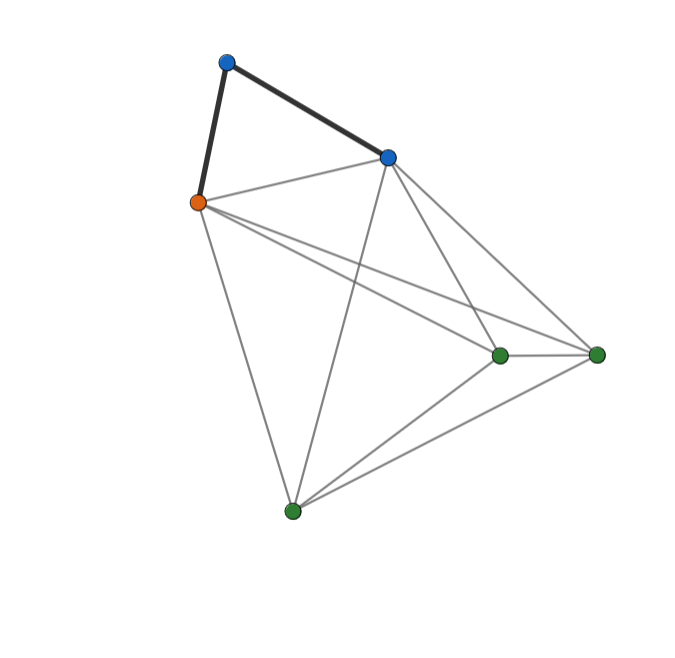
\includegraphics[width=\textwidth]{imagenes/Grafos/Screenshots/Inicial.png}
        \caption{Estdo inicial.}
    \end{subfigure}
    \begin{subfigure}[b]{0.35\textwidth}
        \centering
        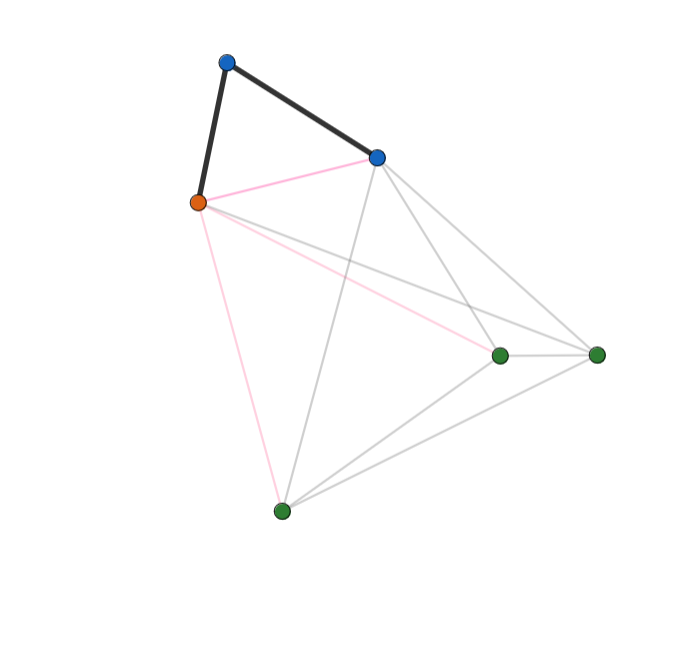
\includegraphics[width=\textwidth]{imagenes/Grafos/Screenshots/Origen1.png}
        \caption{Camninos que llegan al origen.}
    \end{subfigure}
    \begin{subfigure}[b]{0.45\textwidth}
        \centering
        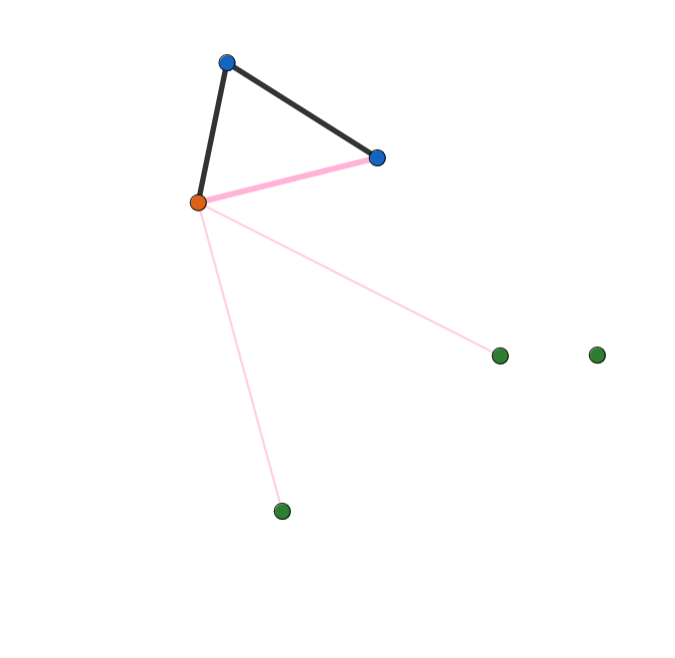
\includegraphics[width=\textwidth]{imagenes/Grafos/Screenshots/Origen2.png}
        \caption{Camino seleccionado.}
    \end{subfigure}
\end{figure}
En (a), (b), (c) estamos aproximando el coste para volver al origen según nuestra función cota. 

\begin{figure}[H]
    \centering
    \begin{subfigure}[b]{0.45\textwidth}
        \centering
        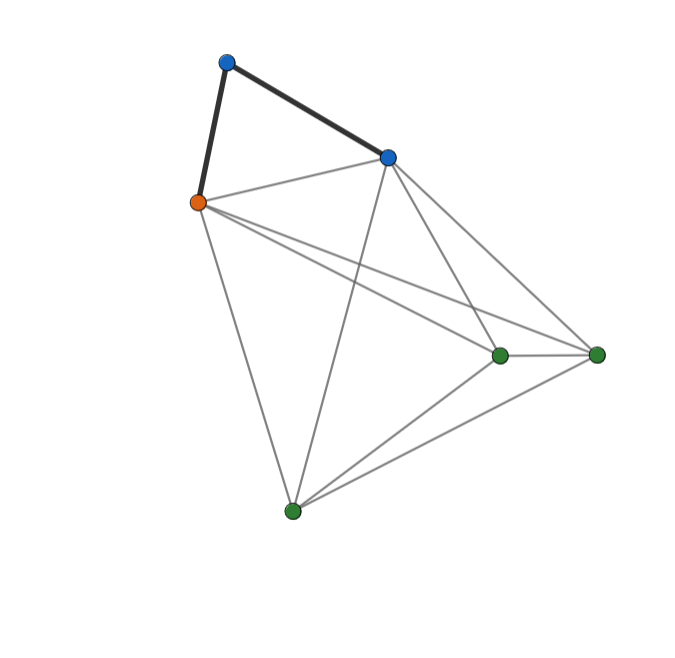
\includegraphics[width=\textwidth]{imagenes/Grafos/Screenshots/Inicial.png}
        \caption{Estado inicial.}
    \end{subfigure}
    %\hfill
    \begin{subfigure}[b]{0.45\textwidth}
        \centering
        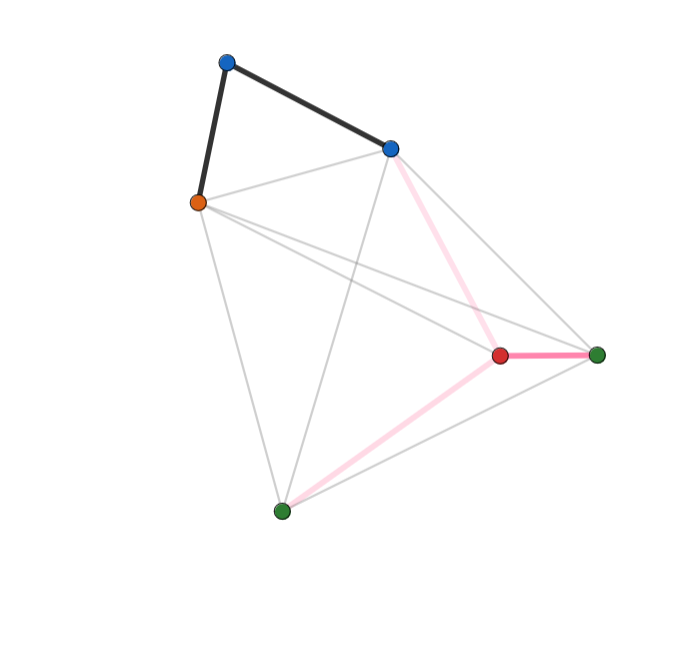
\includegraphics[width=\textwidth]{imagenes/Grafos/Screenshots/Cambio2.png}
        \caption{Caminos candidato para el nodo rojo y camino seleccionado.}
    \end{subfigure}
\end{figure}

En (d) y (e) estamos haciendo lo mismo que lo anterior pero para una ciudad/nodo no visitado (el rojo).

\subsubsection{Detalles de implementación y análisis de eficiencia}

Teniendo en cuenta el diseño previamente explicado nos interesa: 

\begin{enumerate}
    \item Calcular (1)
    \item Calcular para cada ciudad(nodo) el camino mismo para llegar hasta ella desde otra ciudad no visitada o desde la última seleccionada. La suma de todos ellos es (2). 
    \item Calcular el costo mínimo para volver al origen desde una ciudad no visitada o desde la última seleccionada.
\end{enumerate}

Para lo primero solo necesitamos ir acumulando el coste de los caminos de las decisiones ya tomadas. Esto se realiza a medida que se toma las decisiones, luego lo explicaremos más adelante en la implementación de BB y BK, y aquí solo nos limitaremos a (b) y (c), tal y como hemos comentado anteriormete. \\

Por tanto, nuestra función cota se encarga esencialmente de (b) y (c).
Hay un detalle que merece mencionar que es que vamos a considerar la última ciudad a visitar como aun no visitada, pero por visitar, para facilitar la implementación, de allí que la cabecera de nuestra función de cota tenga la siguiente forma: 

\lstinputlisting[language=C++, firstline=140,lastline=144]{codigos/src/Solution.cpp}

En la función sumMinEnter se calcula (2)+(3). Para (2), llama para cada nodo no visitado a la función enter\_min\_cost para calcular (b), recordemos que la suma de todos los (b) es (2). En la última linea 9  se calcula (3) también llamando a enter\_min\_cost para el nodo origen. 

\lstinputlisting[language=C++, firstline=168,lastline=178]{codigos/src/Solution.cpp}

En enter\_min\_cost, dado las decisiones hasta el momento y un nodo no visitado, calcula (b) para dicho nodo. Elige el camino de mínimo coste entre todos los caminos que existen entre el propio nodo con el resto de nodos no visitados (el último nodo visitado en nuestro caso también se considera no visitado). Realiza todos estos cáculos delegando en el 
método shortest\_two\_edges. 

\lstinputlisting[language=C++, firstline=188,lastline=190]{codigos/src/Solution(1).cpp}

Como shortest\_two\_edges tiene eficiencia O(n), donde n es el número de ciudades, luego enter\_min\_cost también. Vemos que sumMinEnter está compuesto por un bucle que en el caso peor llama a enter\_min\_cost n veces, por tanto tiene eficiencia O($n^2$). \\

Veamos el funcionamiento de \verb|shortest_two_edges|:

\lstinputlisting[language=C++, firstline=196, lastline=212]{imagenes/cota3/Solution.cpp}

La idea es calcular los dos mínimos de un vector, lo cual se hace exactamente igual que al calcular el mínimo de un vector, pero añadimos que cada vez que encontremos uno menor que el mínimo, el segundo mínimo pase a ser el mínimo anterior y el mínimo pase a ser el nuevo mínimo encontrado. El otro caso que tenemos que distinguir es que encontremos un elemento mayor que el primer mínimo (mínimo total) pero menor que el segundo mínimo, en cuyo caso se lo asignamos al segundo mínimo. Finalmente, se devuelven ambos en un pair.

\subsection{Funcion de cota 3}
\subsubsection{Diseño y justificación de su validez}
Para la tercera función de cota, la idea que hemos seguido es similar a la de la cota anterior, solo que en lugar de tomar la mínima distancia de entrar a cada nodo, hemos tomado la mínima distancia que supone visitar cada nodo, es decir, entrar y salir de él. Esto es, tomar las dos mínimas aristas de cada nodo y hacer la media. Como para cada nodo habrá que entrar y salir de él, este valor obtenido es cota inferior de pasar por cada nodo, y la suma de este valor para todos los nodos es cota inferior de la solución óptima de una cierta rama, probando con ello su validez. Veámoslo con un ejemplo:

\begin{center}
    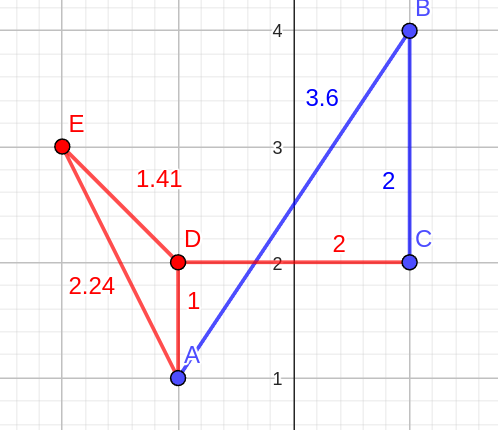
\includegraphics[width=0.5\textwidth]{imagenes/cota3/explicacion.png}
\end{center}

En azul, se marcan los nodos (y los arcos) que ya se han escogido, por tanto esos arcos no se pueden quitar, y en rojo los nodos que quedan por visitar, así como los dos arcos mínimos de cada nodo. 
Hay dos formas de calcular la cota. La primera sería la forma en la que lo hemos explicado: tomar las dos aristas mínimas de cada nodo, hacer la media y sumar. De esta forma nos queda:
\begin{table}[!hbt]
    \centering
    \begin{tabular}{|c|c|c|c|}
            \hline
        Nodos & minEnter & minExit & minVisit \\
        \hline
        A & 1 & 3.6 & $(1+3.6)/2=2.3$ \\
        B & 3.6 & 2 & $(3.6+2)/2=2.8$ \\
        C & 2 & 2 & $(2+2)/2=2$ \\
        D & 1 & 1.41 & $(1+1.41)/2=1.205$ \\
        E & 1.41 & 2.24 & $(1.14+2.24)/2=1.825$ \\
        \hline
        Total & 9.01 & 11.25 & \textbf{10.13} \\
        \hline
    \end{tabular}
\end{table}

Destacar que la cota está por debajo de la solución óptima de la rama (11.25) y que el total de la columna de los minEnter no es ni más ni menos que la cota anterior, pues es la suma de las mínimas aristas de cada nodo, la cual observamos que es más baja que la suma de visitar cada nodo. Esto va a ser siempre así, pues $minVisit(n) \geq minEnter(n) \ \forall n$ al ser $minVisit(n) = \frac{1}{2}(minEnter(n) + minExit(n))$ con $minEnter(n) \leq minExit(n)$. De esta forma se prueba que esta cota es más eficaz. 

La otra forma sería tomar el coste del camino actual, tratar el camino como nodo y sumarle el coste de visitar el camino (promedio de entrar y salir del camino, es decir, mínimo coste de entrar al primer nodo más mínimo coste de salir del último) y por último, sumarle el mínimo coste de visitar cada nodo no visitado:
\[
    total = currentCost + visitTrackCost + sumMinVisit = 5.6 + \frac{1+2}{2} + (1.205+1.825) = \textbf{10.13}
\]

Observamos que ambos resultados coinciden. 

\subsubsection{Detalles de implementación y análisis de eficiencia} \label{subsubsec:ef_fcota3}
La segunda forma comentada de calcular la cota es más sencilla de implementar, por lo que será la forma en que se implemente esta cota:

\lstinputlisting[language=C++, firstline=142, lastline=149]{imagenes/cota3/Solution.cpp}

Donde se ha calculado primero el mínimo de pasar por el camino actual usando dos veces la función \verb|enter_min_cost| ya comentada y luego se ha sumado el resultado de llamar a \verb|sumMinVisit| que se describe a continuación:

\lstinputlisting[language=C++, firstline=176, lastline=185]{imagenes/cota3/Solution.cpp}

Hasta ahora tiene la misma eficiencia que la función \verb|sumMinVisit|. 

Esta función llama para cada nodo no visitado a la función \verb|visit_min_cost| y acumula los resultados en la variable \verb|dist|, por tanto la eficiencia será la eficiencia de \verb|visit_min_cost| por $n$. Veamos cómo funciona esta función:

\lstinputlisting[language=C++, firstline=191, lastline=194]{imagenes/cota3/Solution.cpp}

Observamos que esta función delega su trabajo en la función \verb|shortest_two_edges|, ya comentada, que devuelve las dos aristas más cortas de cada nodo, y les hace la media. Como \verb|shortest_two_edges| tiene eficiencia $O(n)$, la función de cota tiene eficiencia $O(n^2)$ con $n$ el número de ciudades.

\newpage

\section{Algoritmo Backtracking}
\subsection{Diseño y detalles de implementación}

\myparagraph{Diseño}

El algoritmo de \textbf{backtracking} (o \textit{vuelta atrás}) aplicado a este problema consiste en una función recursiva mediante la cual se van explorando todos los nodos (ciudades) siguiendo el algoritmo de recorrido o búsqueda de grafos \textbf{dfs} (\textit{depth first search} o \textit{búsqueda en profundidad}). Al estar explorando todos los caminos posibles (recorriendo todas las ciudades en todos los órdenes posibles) tenemos garantizado que la solución encongtrada será la óptima. 

No obstante,
al ir actualizando siempre nuestra mejor solución hasta el momento e ir construyendo los posibles caminos poco a poco, podemos saber de antemano (gracias a una \textbf{función de cota}) cuando el camino que estamos recorriendo no nos va a dar una solución mejor a la encontrada hasta la fecha. De esta forma, podemos desechar ese camino sin necesidad de procesarlo entero.Tenemos pues que nuestro algoritmo backtracking es el siguiente:

\begin{itemize}
    \item \textbf{Caso base:}
    El camino ya se ha completado (ya se han recorrido todos los nodos/ciudades). Procesamos la solución (si es mejor que la que ya teníamos la actualizamos)
    \item \textbf{Caso general}:
    Todavía no hemos acabado de procesar el camino (estamos visitando una ciudad/nodo intermedio). Procedemos a visitar todas las ciudades que no visitadas (en nuestro camino actual) \textbf{salvo} las que sepamos que no nos van a llevar a una solución mejor que la que ya tenemos (nuestra cota ``poda'' esa ``rama'' al \textbf{no ser factible})
\end{itemize}

\myparagraph{Implementación}

Como hemos mencionado antes en las sección \ref{sec:class_solution}, nos hemos creado una clase \textit{Solution} para un mejor diseño del código,
que comprende los \textit{structs}, funciones de \textbf{cota} y auxiliares
necesarias para implementar tanto \textbf{backtracking} como \textit{branch and bound} con diferentes cotas a elegir. De esta forma favorecemos también la reutilización de código y cotas entre ambas técnicas, al ser muy parecidas entre sí.

\lstinputlisting[language=C++, firstline=15, lastline=24]{codigos/BK/algoritmo.cpp}

En particular, dado que la única diferencia consiste en la implentación del recorrido de las ciudades, hemos creado una clase \textbf{BK\_solution} para \textit{backtracking} que hereda de la clase general Solution e implementa
el método abstracto de \verb|algorithm| acorde a backtracking. Examinemos 
este método más a fondo:

\lstinputlisting[language=C++, firstline=25, lastline=32]{codigos/BK/algoritmo.cpp}

Para empezar contabilizamos todos los nodos generados (no es necesario para la técnica pero nos será útil en el estudio de eficiencia y comparativa de cotas).

Después tenemos el caso base ya explicado, en el cual si ya hemos completado nuestro camino procesamos la nueva solución generada (la comparamos con nuestra mejor solución hasta la fecha y en caso de ser mejor la actualizamos).

\lstinputlisting[language=C++, firstline=34, lastline=44]{codigos/BK/algoritmo.cpp}

En caso de no cumplir los requisitos del caso base, pasamos al caso general.
Procedemos pues a visitar todas las ciudades no visitadas.
Ignoramos la primera ciudad por ser el origen y ya haberla visitado siempre ya que partimos de ahí (esto hará pasar la eficiencia de $O(n!)$ a $O((n-1)!)$).
También, gracias a nuestra función de cota, la cual como ya vimos es llamada por \verb|feasible|, comprobamos si visitar la ciudad $i$-ésima puede darnos una solución mejor a la que tenemos actualmente. En caso negativo la ignoramos también (podamos esta rama, lo que también contabilizamos por el mismo motivo que para los nodos generados).

\lstinputlisting[language=C++, firstline=46, lastline=51]{codigos/BK/algoritmo.cpp}

Una vez tenemos claro que la ciudad no ha sido visitarla y que visitarla ahora nos puede proporcionar una solución mejor a nuestra mejor solución actual, la añadimos a nuestro \textit{camino} (sumamos el coste de la arista al coste total del camino, añadimos la ciudad al camino y la marcamos como visitada). Llamamos a \verb|algorithm| de nuevo para explorar el camino escogido.

\lstinputlisting[language=C++, firstline=53, lastline=56]{codigos/BK/algoritmo.cpp}

Por último, habiendo ya explorado el camino de visitar como siguiente ciudada la $i$-ésima, eliminamos la ciudad del camino para poder considerar otras opciones, es decir, visitar otras ciudades como siguiente en vez de esa. Esto incluye restar el coste añadido por su arista (su ``camino'' desde la última ciudad hasta ella), eliminar la ciudad del camino y desmarcarla como visitada.

\subsection{Analisis de eficiencia}

Dado que el algoritmo \textit{bractraking} lo que hace es explorar todos los caminos posibles formados por $n$ ciudades, esto es, todas las permutaciones de $n-1$ (ya que la primera ciudade siempre es la ciudad origen, 0), tenemos que la eficiencia teórica en el caso pero es $O((n-1)!)$. Esto se debe a que si nuestra función de cota no consigue podar ninguna rama (descartar algún camino), se recorren todos.

Dado que cada conjunto de ciudades es diferente y no existe ninguna condición que verifiquen todos que nos sea de utilidad, no podemos garantizar que ninguna función de poda vaya a podar siempre $x$ nodos como mínimo, dado que siempre puede existe un caso lo suficiente malo en el cual no se pode ningún nodo (ya que est problema es NP-Difícil).

Por tanto, para poder calcular la eficiencia del algoritmo empleando cada función de cota de forma que podamos compararlas entre sí (para saber cuál es mejor en \textbf{media}), haremos lo siguiente: estudiaremos el tiempo que tarda en procesar cada nodo (en base a la función de cota elegida) de forma teórica y el número de nodos que genera de forma empírica.

Veamos primero el tiempo que tarda en procesarse cada nodo. En el caso de \textit{backtraking}, esto consiste en el tiempo que tarda en ejecutarse una llamada a la función \verb|algorithm| (clase \textit{BK\_solution}) sin tener el cuenta el coste añadido por la recurrencia (ya que ese lo contabilizaremos en otros nodos).

\lstinputlisting[language=C++, firstline=24, lastline=32]{codigos/BK/algoritmo.cpp}

El caso base está compuesto de una suma y una comprobación \verb|booleana|
que son $O(1)$ y la eficiencia de \verb|processSolution|. Estudiemos la eficiencia de está función en detalle:

\lstinputlisting[language=C++, firstline=299, lastline=305]{codigos/src/Solution.cpp}

Su eficiencia consiste en operaciones $O(1)$ sumado a la eficiencia de \verb|cycleDistance|. Estudiemos la eficiencia de está función en detalle:

\lstinputlisting[language=C++, firstline=43, lastline=51]{codigos/src/City.cpp}

Tenemos operaciones básicas de sumas y asignaciones que son $O(1)$ y un bucle \mintinline{C++}{for} que se ejecuta $n$ veces donde $n$ es el número de ciudades de \verb|cycle|, es decir de \verb|track|.

En conclusión, la eficiencia del caso base es $O(n)$. Notamos que al haber un \mintinline{C++}{return} en el \mintinline{C++}{if}, el caso base y el caso general son excluyentes. Es decir, es como si tuvieramos una estructura \mintinline{C++}{if-else}.
Aplicando las reglas de cálculo de eficiencias, la eficiencia de la función será el \textbf{máximo} entre la del caso base ya calculado y el caso general.

\lstinputlisting[language=C++, firstline=34, lastline=57]{codigos/BK/algoritmo.cpp}

Pasemos al caso general. Tenemos un bucle \mintinline{C++}{for}
que se ejecuta $n-1$ veces ($n$ número de ciudades), dentro del cual tenemos sumas, asignación y expresiones booleanas que son $O(1)$, la función \verb|feasible| y la llamada recursiva que como mencionamos anteriormente ignoraremos en este caso.
Estudiemos la eficiencia de la función \verb|feasible| en detalle:

\lstinputlisting[language=C++, firstline=96, lastline=103]{codigos/src/Solution.cpp}

Consisten en expresiones booleanas que son $O(1)$ y la función \verb|f_cota|.
Estudiemos la eficiencia de está función en detalle:

\lstinputlisting[language=C++, firstline=105, lastline=130]{codigos/src/Solution.cpp}

Esta función consiste una asignación y una suma (gracias a que vamos almacenando el coste del camino eficientemente en vez de calcularlo constantemente) que son $O(1)$ y una función \texttt{f\_$cota_i$}, que representa la $i$-ésima función de cota implementada.

Por tanto, la eficiencia del cuerpo del \mintinline{C++}{for} es $O(f\_cota_i)$, siendo entonces la complejidad del caso general $O(n \cdot f\_cota_i)$.

En conclusión, el tiempo de procesamiento de un nodo para un caso de entrada de $n$ ciudades es, aplicando la regla del máximo: 
\begin{equation*}
    max\{O(n),O(n \cdot f\_cota_i)\} = O(max\{n,n \cdot f\_cota_i\}) = O(n \cdot f\_cota_i)
\end{equation*}
ya que $O(f\_cota_i)$ será como mínimo $O(1)$. 

De esto deducimos que la eficiencia de \verb|algorithm| (clase BK\_solution) en función del número de nodos generados y la cota aplicada es:
\begin{equation*}
    O(n \cdot f\_cota_i \cdot num\_nodos)
\end{equation*}

Notamos que para algunas cotas, se tiene la necesidad de realizar una serie de cálculos previos para evitar que se estén recalculando constantemente y que sea más eficiente. Estos cálculos se realizan aparte (previamente) y no dependen del número de nodos. Consideramos en esos casos reemplazar la fórmula mencionada arriba por esta otra:
\begin{equation*}
    O(n \cdot f\_cota_i \cdot num\_nodos) + O(calculos\_previos)
\end{equation*}

Por último, si queremos saber la eficiencia del algoritmo \textbf{backtracking}, examinamos primero el constructor de la clase \verb|BK_solution| (heredado de la clase \verb|Solution|).

\lstinputlisting[language=C++, firstline=27, lastline=32]{codigos/src/Solution.cpp}

Ahí tenemos operaciones básicas $O(1)$, la función \verb|TSP_greedy| que ya vimos en la práctica anterior que era $O(n^{2})$ (se corresponde con la primera versión) y la función \verb|cyleDistance| que ya hemos visto que es $O(n)$. La eficiencia del constructor es entonces $O(n^{2})$.

Finalemente estudiemos la función \verb|solve|, que es la que llama a la función \verb|algorithm| con el algoritmo \textbf{backtracking} implementado que hemos visto antes.

\lstinputlisting[language=C++, firstline=71, lastline=72]{codigos/src/Solution.cpp}
\lstinputlisting[language=C++, firstline=77, lastline=81]{codigos/src/Solution.cpp}

Todas la operaciones son $O(1)$ salvo la función \verb|algorithm|. En conclusión, la \textbf{eficiencia} del algorithmo \textbf{backtracking} es:
\begin{equation*}
    O(n \cdot f\_cota_i \cdot num\_nodos + n^{2})
\end{equation*}

Procedamos ahora a \textbf{aproximar} $num\_nodos$ (número de nodos generados) mediante una función (preferiblemente un polinomio) $p(n)$ para cada función de cota. Juntando la expresión de esta función con la fórmula obtenida y la eficiencia teórica de cada cota daremos con una \textbf{aproximación} de la complejidad temporal para cada cota.

\subsubsection{Funcion cota 1}

\myparagraph{Eficiencia teórica}

Recordamos que la eficiencia teórica de nuestra función de cota 1 vista en la sección \ref{subsubsec:ef_fcota1}, es $O(1)$, con un añadido de cálculos previos que constituyen $O(n^{2}log\:n^{2})$.

Sustituyendo, tenemos que la eficiencia de \textbf{backtracking} para la cota 1 en función del número de nodos generados es: 
\begin{equation*}
    O(n \cdot f\_cota_i \cdot num\_nodos + n^{2}) + O(calculos\_previos) = 
    O(n \cdot num\_nodos + n^{2}) + O(n^{2}) = O(n \cdot num\_nodos + n^{2})
\end{equation*}

\myparagraph{Aproximación número de nodos}
Estudiemos ahora el número de nodos generados (en función del tamaño de la entrada), tratando de aproximar esta función \textbf{híbridamente} mediante \textbf{regresiones}. Dado que no 
tenemos en principio ninguna expresión teórica de base que nos indique de que orden puede ser está función, hemos probado diversos ajustes híbridamente hasta dar con alguno que ajuste bien nuestra función.

\begin{figure}[H]
    \centering
    \begin{subfigure}[b]{0.45\textwidth}
        \centering
        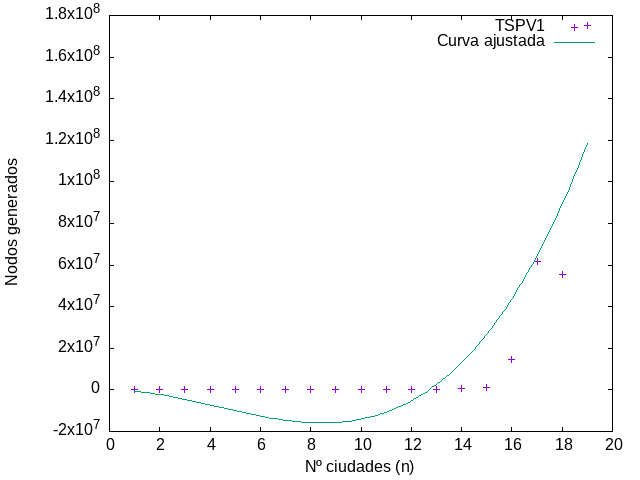
\includegraphics[width=\textwidth]{imagenes/cota1/eficiencia_nodos_bk/CurvaAjustada_n3.png}
        \caption{Cúbica}
    \end{subfigure}
    \begin{subfigure}[b]{0.45\textwidth}
        \centering
        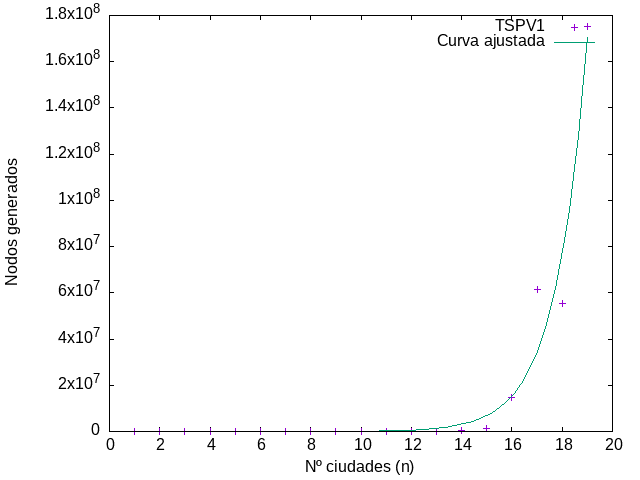
\includegraphics[width=\textwidth]{imagenes/cota1/eficiencia_nodos_bk/CurvaAjustada_exp.png}
        \caption{Exponencial $O(e^{n})$}
    \end{subfigure}
\end{figure}
\begin{figure}[H]
\centering
    \begin{subfigure}[b]{0.45\textwidth}
        \centering
        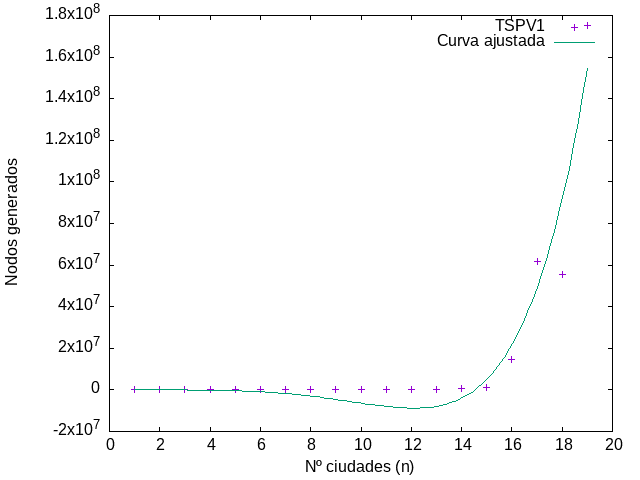
\includegraphics[width=\textwidth]{imagenes/cota1/eficiencia_nodos_bk/CurvaAjustada_n6.png}
        \caption{Polinomio de grado 6}
    \end{subfigure}
    \begin{subfigure}[b]{0.45\textwidth}
        \centering
        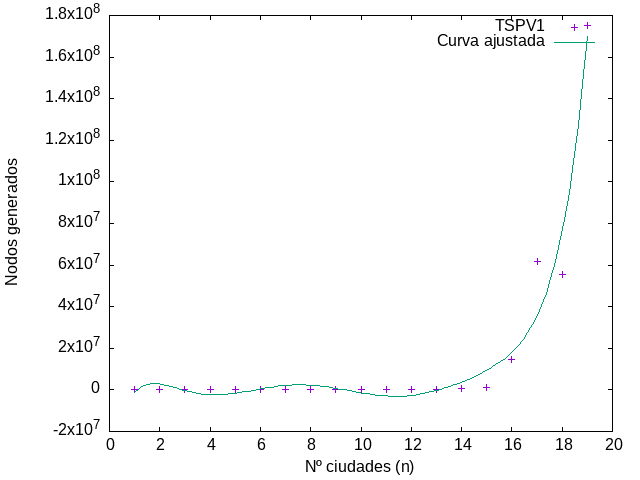
\includegraphics[width=\textwidth]{imagenes/cota1/eficiencia_nodos_bk/CurvaAjustada_n7.png}
        \caption{Polinomio de grado 7}
    \end{subfigure}
    \begin{subfigure}[b]{0.45\textwidth}
        \centering
        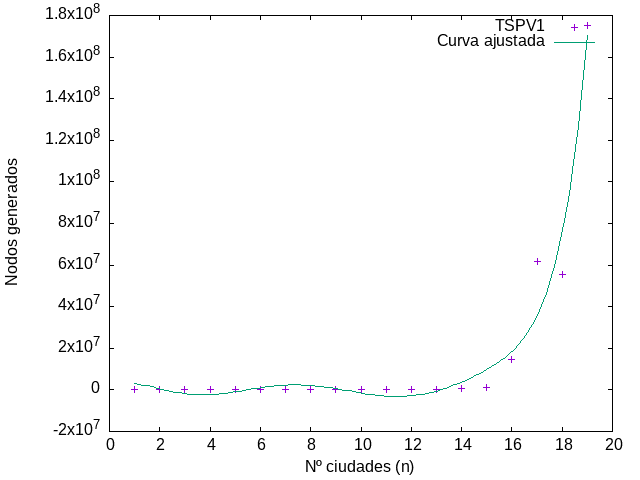
\includegraphics[width=\textwidth]{imagenes/cota1/eficiencia_nodos_bk/CurvaAjustada_n8.png}
        \caption{Polinomio de grado 8}
    \end{subfigure}
    \begin{subfigure}[b]{0.45\textwidth}
        \centering
        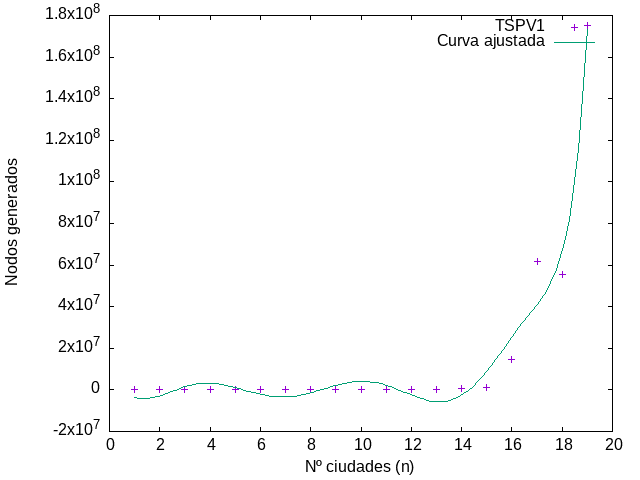
\includegraphics[width=\textwidth]{imagenes/cota1/eficiencia_nodos_bk/CurvaAjustada_n9.png}
        \caption{Polinomio de grado 9}
    \end{subfigure}
\end{figure}

Observando las gráficas con los ajustes realizados, podemos ver a la hora de aproximar la función con un polinomio, empezamos a obtener resultados relativamente decentes a partir del grado 7, siendo muy bien ajustada para un polinomio de grado 9. Por otro lado, la función exponencial también ajusta bien a esta función. Veamos que tan buenas son las bondades de estos ajustes.
\begin{itemize}
    \item Para la exponencial:
\lstinputlisting[firstline=422, lastline=427,numbers=none]{imagenes/cota1/eficiencia_nodos_bk/fit.log}
     \item Para el polinomio de grado 9:
\lstinputlisting[firstline=370, lastline=383,numbers=none]{imagenes/cota1/eficiencia_nodos_bk/fit.log}
\end{itemize}

Comparando las \textbf{varianzas residuales}, tenemos que la función exponencial ajusta mejor a nuestra función que el polinomio de grado 9, no obstante nos quedaremos con este último dado que la diferencia no es muy significativa y los polinomios suelen ser más ventajosos. Notamos que a pesar de ver un buen ajuste en a gráfica, la varianza residual sigue siendo considerablemente \textbf{alta}. Esto es de esperarse, dado que el número de nodos generados depende mucho del caso en particular de entrada, y no solo del tamaño de la entrada (aunque este claramente también influye).

Tomaremos entonces como función de aproximación del número de nodos generados en base a $n$ a una de orden $O(n^{9})$. Sustituyendo $num\_nodos$
en la fórmula previamente deducida nos queda que la eficiencia teórica es:
\begin{equation*}
    O(n\cdot num\_nodos + n^{2}) = O(n\cdot n^{9} + n{2}) = O(n^{10})
\end{equation*}

\myparagraph{Eficiencia empírica}

Veamos ahora la eficiencia empírica de nuestro algoritmo backtracking para la cota 1.

\begin{figure}[H]
    \centering
    \begin{subfigure}[b]{0.45\textwidth}
        \centering
        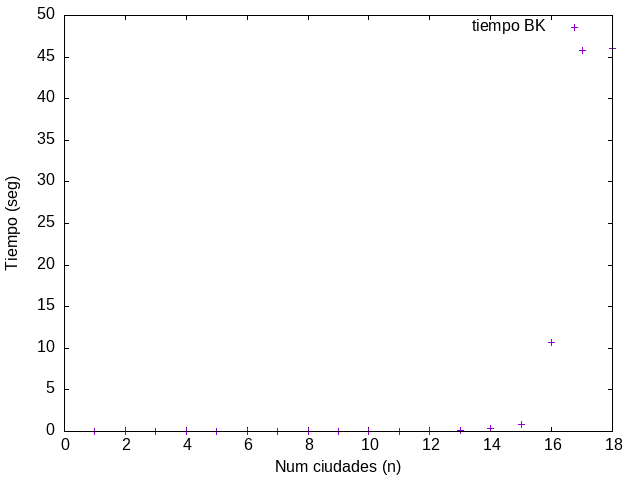
\includegraphics[width=\textwidth]{imagenes/cota1/ef_bk/TSP_BK_empirica_points.png}
        \caption{Puntos}
    \end{subfigure}
    \begin{subfigure}[b]{0.45\textwidth}
        \centering
        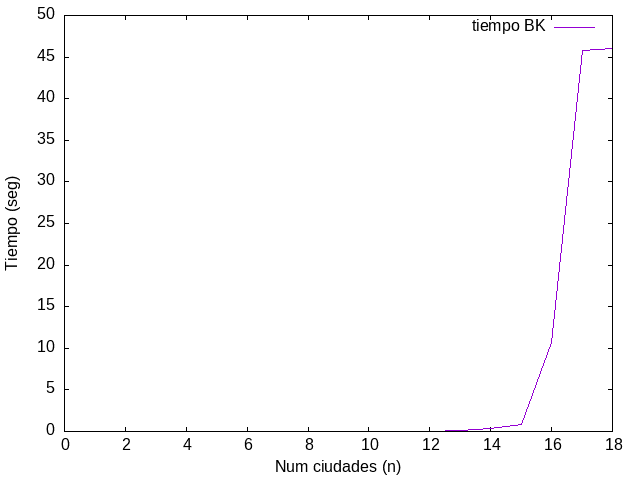
\includegraphics[width=\textwidth]{imagenes/cota1/ef_bk/TSP_BK_empirica_lines.png}
        \caption{Líneas}
    \end{subfigure}
\end{figure}

Podemos ver que el algoritmo bracktracking crece \textbf{muy} rápidamente 
para la cota 1.

\myparagraph{Eficiencia híbrida}

Procedamos ahora a ajustar los datos obtenidos para la eficiencia empírica mediante la expresión obtenida en la eficiencia teórica, $O(n^{10})$.

\begin{figure}[!hbt]
    \centering
    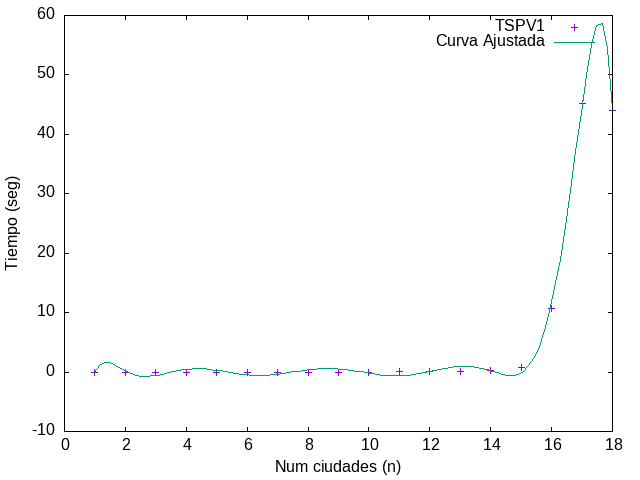
\includegraphics[width=0.5\textwidth]{imagenes/cota1/ef_bk/ef_ajustada_n10.png}
    \caption{Tiempo ajustado por polinomio de grado 10}
    \label{fig:enter-label}
\end{figure}

Veamos la varianza residual del ajuste:

\begin{lstlisting}[numbers=none]
variance of residuals (reduced chisquare) = WSSR/ndf   : 0.658663

Final set of parameters            Asymptotic Standard Error
=======================            ==========================
a0              = -62.7335         +/- 26.75        (42.64%)
a1              = 154.11           +/- 61.05        (39.62%)
a2              = -145.847         +/- 53.06        (36.38%)
a3              = 71.9815          +/- 23.95        (33.28%)
a4              = -20.9532         +/- 6.38         (30.45%)
a5              = 3.82151          +/- 1.067        (27.92%)
a6              = -0.44809         +/- 0.1151       (25.68%)
a7              = 0.0337065        +/- 0.007988     (23.7%)
a8              = -0.00156995      +/- 0.0003446    (21.95%)
a9              = 4.11677e-05      +/- 8.399e-06    (20.4%)
a10             = -4.64101e-07     +/- 8.835e-08    (19.04%)

\end{lstlisting}

Como podemos ver, el ajuste está lejos de ser perfecto, como era de esperarse por no poder ajustar bien el número de nodos generados, pero aproxima bastante bien la complejidad temporal de backtracking para la cota 1, como se puede ver de la varianza residual.

\subsubsection{Funcion cota 2}

\myparagraph{Eficiencia teórica-híbrida}
Teniendo en cuenta que esta función de cota tiene eficiencia $O(n^2)$, 
veamos si podemos aproximar el número de nodos que se generan por el Backtraking se puede aproximar por alguna función. Ejecuntado el algoritmo con diferentes tamaños de entrada, entre 4 y 19, obtenemos las siguientes gráficas:


\begin{figure}[H]
    \centering
    \begin{subfigure}[b]{0.45\textwidth}
        \centering
        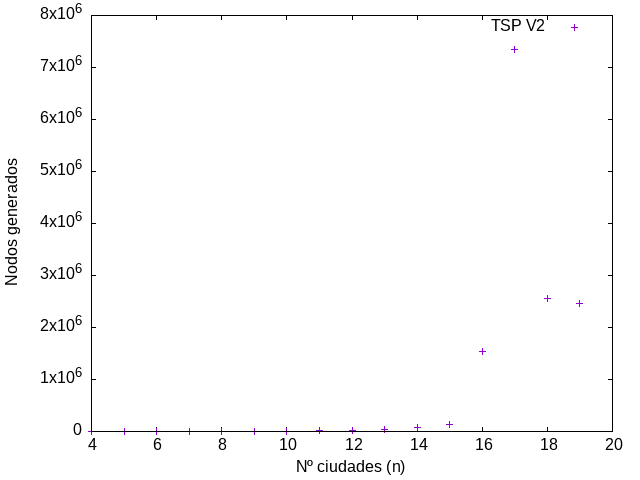
\includegraphics[width=\textwidth]{Sucio_Olga/Data/salidaSoloPuntos.png}
        \caption{Puntos.}
    \end{subfigure}
    %\hfill
    \begin{subfigure}[b]{0.45\textwidth}
        \centering
        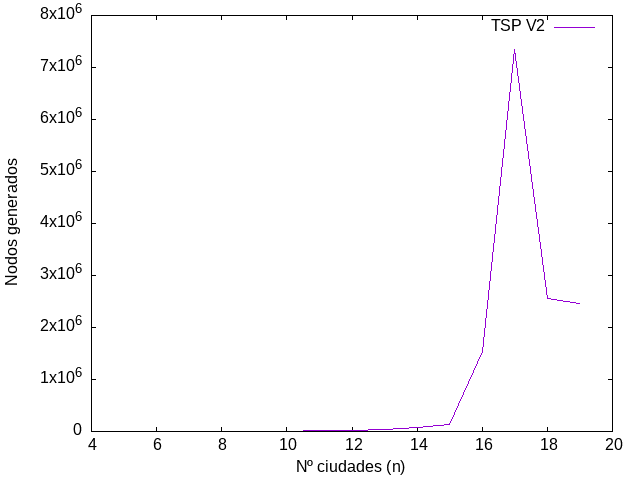
\includegraphics[width=\textwidth]{Sucio_Olga/Data/salidaSoloLineas.png}
        \caption{Lineas.}
    \end{subfigure}
\end{figure}

Podemos observar que el número de nodos generados  no es estable y fluctúa mucho, esto es debido a que el algoritmo lista las distintas posibilidad en un orden sistemático y nuestra función de poda no puede influir en esto, solo puede ayudar a que se generen menos nodos, posibilitando así que la solución óptima puede estar entre uno de los últimos nodos generados. \\

Aproximando el comportamiento por diferentes tipos de funciones, desde polinómicas y exponenciales hasta factoriales, obtenemos: 

\begin{figure}[H]
    \centering
    \begin{subfigure}[b]{0.45\textwidth}
        \centering
        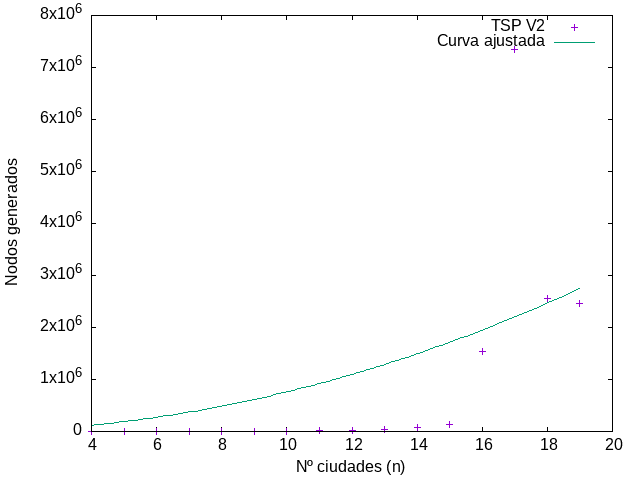
\includegraphics[width=\textwidth]{Sucio_Olga/Data/CurvaAjustadaCuadratica.png}
        \caption{Cuadratica con $f(x)=7625.1 x^2$}
    \end{subfigure}
    %\hfill
    \begin{subfigure}[b]{0.45\textwidth}
        \centering
        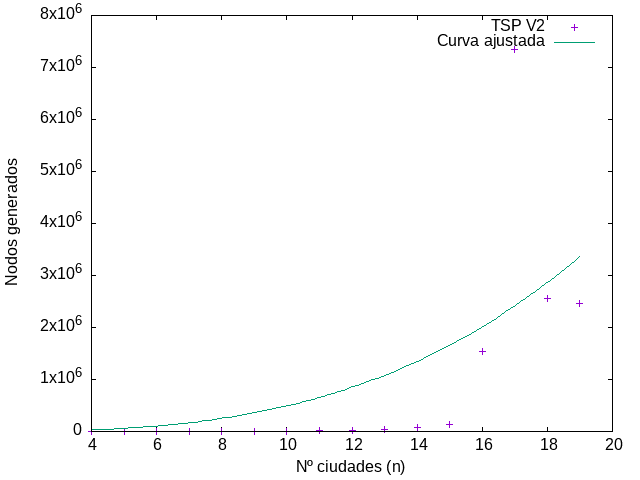
\includegraphics[width=\textwidth]{Sucio_Olga/Data/CurvaAjustadaCubica.png}
        \caption{Cubica con $f(x)=491.71x^3$}
    \end{subfigure}
    %\hfill
    \begin{subfigure}[b]{0.45\textwidth}
        \centering
        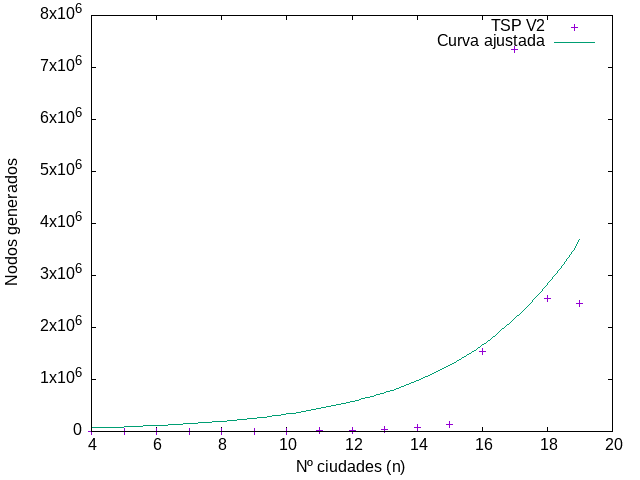
\includegraphics[width=\textwidth]{Sucio_Olga/Data/CurvaAjustadaExponencial.png}
        \caption{Exponencial con $f(x)=23374 e^{0.27x}$}
    \end{subfigure}
    %\hfill
    \begin{subfigure}[b]{0.45\textwidth}
        \centering
        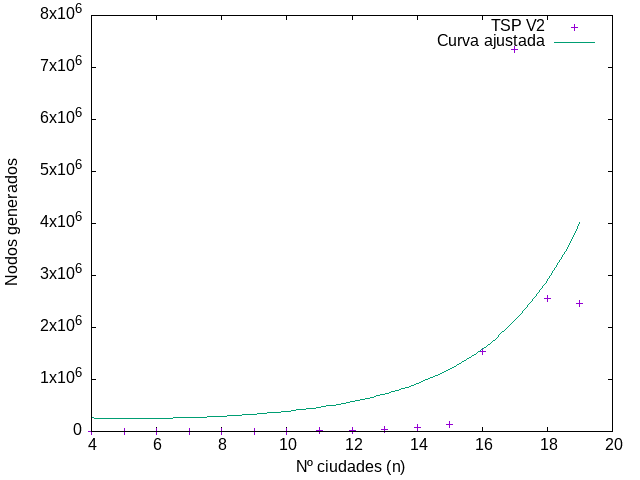
\includegraphics[width=\textwidth]{Sucio_Olga/Data/CurvaAjustadaFactorial.png}
        \caption{Factorial con $f(x)=282197\Gamma(0.23(x+1))$}
    \end{subfigure}
\end{figure}

Visualmente podemos ver que ninguna de ellas aproximan decentemente a 
los resultados obtenidos y analizando los errores de la regresión confirman lo anterior, todos ellos tienen una varianza residual del orden de $10^{12}$ (más detalles en el fichero BK/fit.log). \\

Tomaremos como función de aproximación de nodos la función exponencial 
ya que de entre todas las mediocres regresiones es la mejor. Por tanto, combinando todo tenemos que si T(n) es la eficiencia del BK, entonces
$T(n) \in O(n^3 e^n + n^2) = O(n^3 e^n)$. 

\myparagraph{Eficiencia empírica e híbrida}

Recogiendo diferentes tiempos de ejecución con datos de entrada entre 4-19 ciudades obtenemos las siguientes gráficas: 

\begin{figure}[H]
    \centering
    \begin{subfigure}[b]{0.45\textwidth}
        \centering
        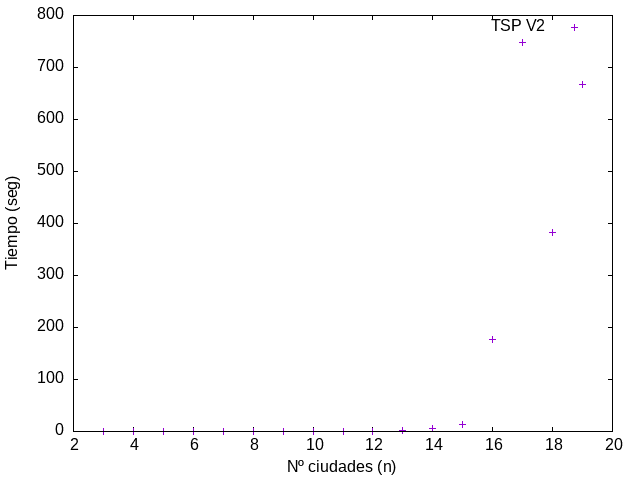
\includegraphics[width=\textwidth]{Sucio_Olga/DatosBK/salidaSoloPuntos.png}
        \caption{Puntos.}
    \end{subfigure}
    %\hfill
    \begin{subfigure}[b]{0.45\textwidth}
        \centering
        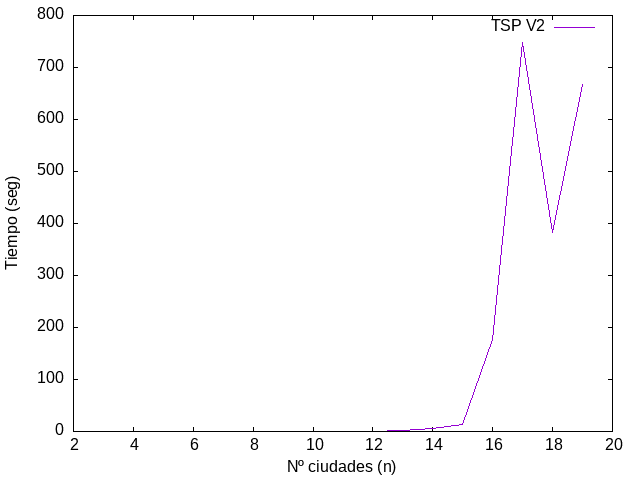
\includegraphics[width=\textwidth]{Sucio_Olga/DatosBK/salidaSoloLineas.png}
        \caption{Lineas}
    \end{subfigure}
\end{figure}

Podemos ver que el comportamiento es muy irregular e inestable, ya que tiene un factor del azar en su comportamiento, pero refleja a la perfección el crecimiento en tiempo de la ejecución a medida que aumentan los tamaños de entrada. 

Ahora ajustamos con una curva del tipo $f(x)=a x^3 e^{b x}$, tipo de función obtenida teorica-empíricamente, y obtenemos el siguiente resultado: 

\begin{figure}[H]
    \centering
    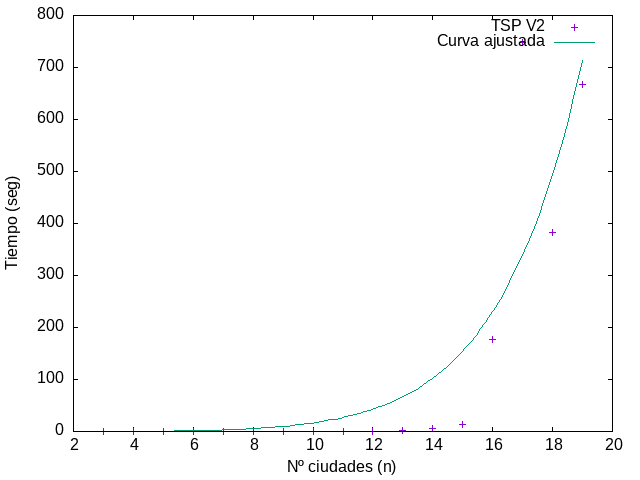
\includegraphics[width=0.45\textwidth]{Sucio_Olga/DatosBK/CurvaAjustadaExponencial.png}
    \caption*{$f(x)=0.00213 x^3 e^{0.205x}$}
\end{figure}

Analicemos la calidad de este ajuste: 
\lstinputlisting[language=C++, firstline=24, lastline=32]{Sucio_Olga/DatosBK/fit.log}

Podemos ver que tanto la varianza residual como el porcentaje de error asintótico estándar toman valores muy altos, esto quiere decir que nuestro ajuste no es preciso, tal y como se puede apreciar en la gráfica. Podemos atribuir dicho fracaso de la regresión al comportamiento relativamente impredictible de nuestro algoritmo, ya que depende de según dónde se encuentre la solución óptima, tendremos que recorrer más o menos nodos. 

\subsubsection{Funcion cota 3} \label{subsubsection:nodes_f_cota3}

Como ya se comentó en la sección \ref{subsubsec:ef_fcota3}, la función de cota 3 tiene eficiencia cuadrática en el número de ciudades, luego la eficiencia del algoritmo backtracking será de:
\[
    O(n^3 \cdot num\_nodos)
\]
Pues ya será mayor que $n^2$. Luego nuestro objetivo es estudiar el número de nodos que se generan. \\
Lo ideal sería encontrar una función devuelva el número de nodos generados en función del número de ciudades, no obstante eso no es posible, pues depende mucho del número de casos, como se muestra en la tabla:

\begin{table}[h!]
\centering
\begin{tabular}{|c|c|}
\hline
\textbf{Ciudades} & \textbf{Nodos generados} \\
\hline
1 & 1 \\
\hline
2 & 2 \\
\hline
3 & 5 \\
\hline
4 & 12 \\
\hline
5 & 25 \\
\hline
6 & 40 \\
\hline
7 & 169 \\
\hline
8 & 482 \\
\hline
9 & 600 \\
\hline
10 & 1253 \\
\hline
11 & 1297 \\
\hline
12 & 426 \\
\hline
13 & 1209 \\
\hline
14 & 3015 \\
\hline
15 & 8809 \\
\hline
16 & 20653 \\
\hline
17 & 245151 \\
\hline
18 & 27792 \\
\hline
19 & 8702 \\
\hline
\end{tabular}
\caption{Nodos generados para la cota 3 en el algoritmo backtracking}
\label{tab:datos}
\end{table}

Lo máximo que se puede hacer es buscar una regresión que aproxime lo máximo posible a un muestreo, que en nuestro caso sera $1 \leq n \leq 19$. Se ha probado con $n^p$ para $1 \leq p \leq 9$ y con una regresión exponencial, los mejores resultados se han obtenido para $n^6$ y para $n^9$, como se muestra a continuación:

\begin{figure}[H]
    \centering
    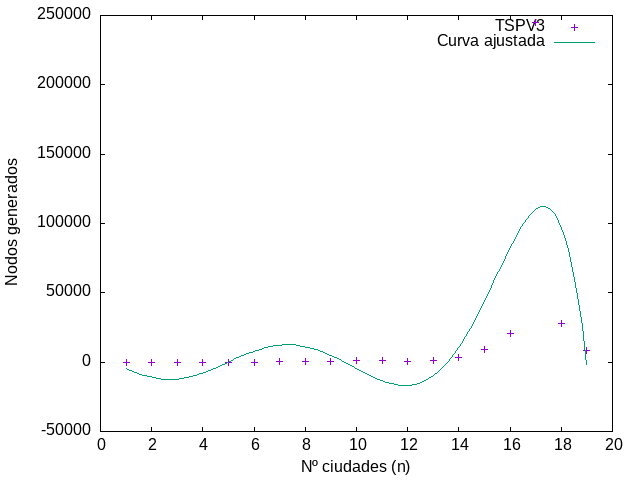
\includegraphics[width=0.7\textwidth]{imagenes/cota3/CurvaAjustada_n6_bk.png}
    \caption*{$f(x)=-0.622198 \cdot x^6 + 29.2992 \cdot x^5 -484.335 \cdot x^4 + 3294.8 \cdot x^3 -7637.95 \cdot x^2 + 1.25944 \cdot x + 1.02235$}
\end{figure}

\lstinputlisting[language=C++, firstline=223, lastline=237]{imagenes/cota3/fit.log}

\begin{figure}[H]
    \centering
    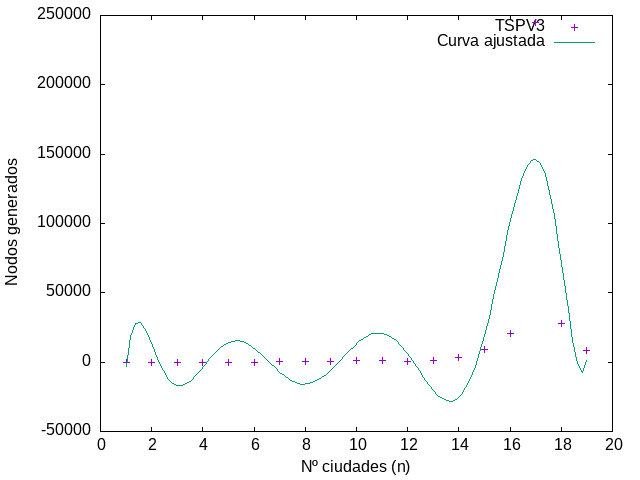
\includegraphics[width=0.7\textwidth]{imagenes/cota3/CurvaAjustada_n9_bk.png}
    \caption*{$f(x)=0.0170416 \cdot x^9 - 1.49802 \cdot x^8 + 55.3892 \cdot x^7 -1121.19  \cdot x^6 + 13550.3 \cdot x^5 -100071 \cdot x^4 + 443999 \cdot x^3 -1116220 \cdot x^2 + 1401350 \cdot x -644323$}
\end{figure}

\lstinputlisting[language=C++, firstline=367, lastline=384]{imagenes/cota3/fit.log}


Observamos que las gráficas no aproximan ni por asomo a los puntos, lo cual lo refleja el alto valor de la varianza residual, aunque de todas las regresiones que se han hecho son las dos con varianza residual más baja. Es por eso que nos quedaremos con estas regresiones, en particular con la mejor de ellas: $n^9$. Siguiendo este modelo podríamos decir que nuestro algoritmo backtracking con la cota 3 tiene una eficiencia de $O(n^{12})$, aunque esto no tenga ningún sentido. \\

Aún así vamos a ajustar la gráfica de los tiempos por un polinomio de grado 12 y ver qué ocurre:

\lstinputlisting[language=C++, firstline=24, lastline=43]{imagenes/cota3/fittiempos.log}

\begin{figure}[H]
    \centering
    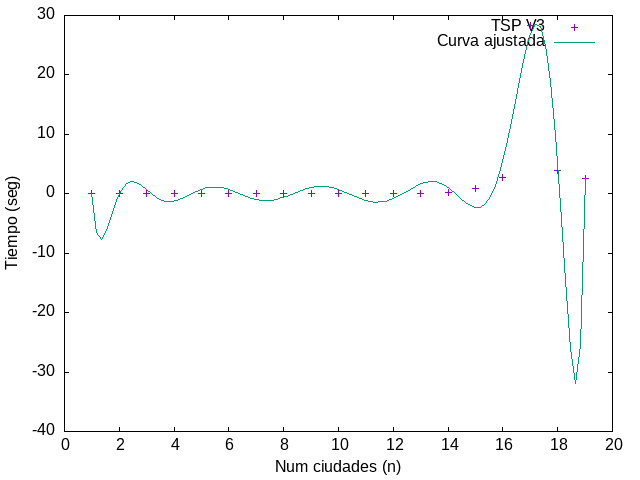
\includegraphics[width=0.7\textwidth]{imagenes/cota3/tiempos_bk.png}
    \caption*{$f(x)=2.88407 \cdot 10^{-8} \cdot x^{12} -3.32313 \cdot 10^{-6} \cdot x^{11} + 0.000169223 \cdot x^{10} -0.00501725  \cdot x^9 + 0.0960471 \cdot x^8 -1.24438 \cdot x^7 +11.1218  \cdot x^6 -68.6027 \cdot x^5 +287.395 \cdot x^4 -789.242  \cdot x^3 +1331.53 \cdot x^2 -1219.1 \cdot x +448.07$}
\end{figure}

Aunque la varianza residual nos haya salido considerablemente menor, insistimos en que esta forma de modelizar el tiempo en función del número de ciudades no tiene mucho sentido al no seguir el número de nodos una monotonía respecto al número de ciudades.

\newpage
\section{Algoritmo Branch and Bound}

\subsection{Diseño y detalles de implementación}

\myparagraph{Introducción}

El algoritmo Branch and Bound (BB) es una técnica de búsqueda heurística ampliamente utilizada para resolver problemas de optimización combinatoria, como el problema del vendedor ambulante (TSP). Al igual que el algoritmo Backtracking (BK), el objetivo de BB es encontrar la ruta óptima que visita todas las ciudades y regresa al punto de partida. Sin embargo, BB utiliza una estrategia diferente para explorar el espacio de soluciones y, en general, es más eficiente que BK para problemas de gran tamaño con cotas lo suficiente buenas.
\myparagraph{Funcionamiento del algoritmo}
El algoritmo BB se basa en la idea de dividir el problema en subproblemas más pequeños y resolverlos, al menos de forma natural, recursivamente. \footnote{Si bien en este caso lo hemos implementado de forma iterativa con una cola con prioridad} Cada subproblema representa una parte del espacio de búsqueda, y la solución óptima del problema original se encuentra al combinar las soluciones óptimas de sus subproblemas.

Para implementar el algoritmo BB, se utilizan dos técnicas principales:
\begin{itemize}
    \item Ramificación: Se divide el problema en subproblemas más pequeños seleccionando una variable de decisión y asignándole diferentes valores.
    \item Acotaciones: Se calculan cotas superior e inferior para el valor óptimo de cada subproblema. Si la cota superior de un subproblema es menor que la cota inferior de otro subproblema, el primer subproblema se puede descartar, ya que no puede contener la solución óptima.
\end{itemize}

\myparagraph{Ventajas del algoritmo BB}
\begin{itemize}
    \item Eficiencia: El algoritmo BB puede ser más eficiente que el algoritmo BK para problemas de gran tamaño con cotas eficaces, ya que al implementarse con una \verb|priority_queue| tenemos que procesamos antes las soluciones que serán posiblemente mejores, provocando esto que se realicen (probablemente) más podas que en backtracking (al tener una cota superior menor y por tanto mejor).
    \item Flexibilidad: BB se puede adaptar a diferentes problemas de optimización combinatoria con modificaciones menores.
\end{itemize}
\myparagraph{Desventajas del algoritmo BB}
\begin{itemize}
    \item Complejidad: BB puede ser más complejo de implementar que BK.
    \item Memoria: BB puede requerir más memoria que BK, ya que almacena información sobre las ramas del árbol de búsqueda que se han explorado. (Y más en este caso concreto, almacenando los nodos en una priority\_queue)
\end{itemize}
\myparagraph{Conclusión}

El algoritmo BB es una técnica de búsqueda heurística poderosa que se puede utilizar para resolver problemas de optimización combinatoria complejos, como el TSP. Su eficiencia y flexibilidad lo convierten en una herramienta valiosa para una amplia gama de aplicaciones.

\myparagraph{Comparación con el algoritmo Backtracking (BK)}

El algoritmo BB es similar al algoritmo Backtracking (BK) en el sentido de que ambos exploran sistemáticamente el espacio de búsqueda para encontrar la solución óptima. Sin embargo, existen algunas diferencias clave entre los dos algoritmos:
\begin{itemize}
    \item Recorrido del árbol de búsqueda: El algoritmo BB utiliza un recorrido de la estructura de árbol de búsqueda similar al \textbf{bfs}. Se diferencia en que en este caso usamos una \verb|priority_queue| en vez de una \verb|queue| normal. Esto constrasto con el recorrido realizado en backtracking que era justamente un \textit{dfs}.
    \item Eficiencia: En general, el algoritmo BB se considera más eficiente que el algoritmo BK para problemas de gran tamaño con una buena cota.

\end{itemize}
En resumen, el algoritmo BB es una herramienta más versátil y eficiente que el algoritmo BK para resolver problemas de optimización combinatoria complejos.

\myparagraph{Implementación}



Como hemos mencionado antes en la sección \ref{sec:class_solution}, nos hemos creado una clase \textit{Solution} para un mejor diseño del código,
que comprende los \textit{structs}, funciones de \textbf{cota} y auxiliares
necesarias para implementar tanto \textit{backtracking} como \textbf{branch and bound} con diferentes cotas a elegir. De esta forma favorecemos también la reutilización de código y cotas entre ambas técnicas, al ser muy parecidas entre sí.

\lstinputlisting[language=C++, firstline=18, lastline=24]{codigos/BB/algoritmo.cpp}

En particular, dado que la única diferencia consiste en la implementación del recorrido de las ciudades, hemos creado una clase \textbf{BB\_solution} para \textit{branch and bound} que hereda de la clase general Solution e implementa
el método abstracto de \verb|algorithm| acorde a branch and bound. Examinemos 
este método más a fondo:

\lstinputlisting[language=C++, firstline=27, lastline=34]{codigos/BB/algoritmo.cpp}

Para empezar, creamos la priority\_queue en la que almacenaremos los nodos según su cota inferior, añadimos el primer nodo y comenzamos a pocesar:
Almacenamos en e\_node el nodo que toca según la cola (en la primera iteración el primero) y lo sacamos de la cola.
\lstinputlisting[language=C++, firstline=36, lastline=41]{codigos/BB/algoritmo.cpp}
Después, si hemos superado el costo de nuestra mejor solución, podemos olvidarnos de este camino y seguir con el siguiente.\newline
Suponiendo que no es así, tenemos el caso base ya explicado, en el cual si ya hemos completado nuestro camino procesamos la nueva solución generada (la comparamos con nuestra mejor solución hasta la fecha y en caso de ser mejor la actualizamos).

\lstinputlisting[language=C++, firstline=43, lastline=49]{codigos/BB/algoritmo.cpp}

En caso de no cumplir los requisitos del caso base, pasamos al caso general.
Procedemos pues a visitar todas las ciudades no visitadas.
Ignoramos la primera ciudad por ser el origen y ya haberla visitado siempre ya que partimos de ahí (esto hará pasar la eficiencia de $O(n!)$ a $O((n-1)!)$).
También, gracias a nuestra función de cota, la cual como ya vimos es llamada por \verb|feasible|, comprobamos si visitar la ciudad $i$-ésima puede darnos una solución mejor a la que tenemos actualmente. En caso negativo la ignoramos también (podamos esta rama, lo que también contabilizamos por el mismo motivo que para los nodos generados).



\lstinputlisting[language=C++, firstline=50, lastline=56]{codigos/BB/algoritmo.cpp}

Una vez tenemos claro que la ciudad no ha sido visitada y que visitarla ahora nos puede proporcionar una solución mejor a nuestra mejor solución actual, la añadimos a nuestro \textit{camino} (sumamos el coste de la arista al coste total del camino, añadimos la ciudad al camino y la marcamos como visitada). 
Además la añadimos a nuestra priority\_queue para que en la siguiente iteración se procese (y así seguir recorriendo este camino)


\subsection{Analisis de eficiencia}

Ahora vamos a estudiar la eficiencia de este algoritmo utilizando distintas funciones de cota. En primer lugar, vamos a estudiar la cantidad de nodos 
generados en relación al número de ciudades. Teóricamente en el caso peor este debería ser (n-1)! si n fuese el número de ciudades, pero dependiendo de lo bueno que sea la función de cota utilizada esta cantidad puede verse reducida. Por tanto, el objetivo es encontrar una función p(n) (preferiblemente un polinomio) que aproxime dicha cantidad de nodos. 

Una vez determinado lo anterior, notemos que el algoritmo esta compuesto en esencia de un bucle while que itera p(n) veces, ya que no para hasta que la cola que guarda todos los nodos vivos esté vacía. Su cuerpo está formado por, a parte de sentencias simples de orden O(1), por otro bucle for que itera n-1 veces y llama a la función de cota en cada iteración. También hay una inserción en la cola de prioridad en el bucle, pero como no siempre ocurre, ya que hay un 'continue' que le precede, concluimos que esta inserción ocurre p(n) veces (ya que lo que se insertan son nodos factibles), independientemente de las iteraciones del bucles, y como cada inserción es del orden logarítmico, las inserciones en total tiene coste $p(n)\log{p(n)}$. Por tanto, si llamamos a la eficiencia de la función cota q(n) y T(n) a la eficiencia del algoritmo de Branch And Bound, aplicando la regla del máximo y de la suma tenemos: 

\[
    T(n) = p(n)(n-1)q(n) + p(n)\log{p(n)} = p(n)((n-1)q(n) +   \log{p(n)}) = p(n)(n\:q(n) +   \log{p(n)})
\]

\subsubsection{Funcion cota 1}

\myparagraph{Eficiencia teórica}

Recordamos que la eficiencia teórica de nuestra función de cota 1 vista en la sección \ref{subsubsec:ef_fcota1}, es $O(1)$, con un añadido de cálculos previos que constituyen $O(n^{2}log\:n^{2})$.

Sustituyendo la eficiencia de nuestra cota ($q(n) = 1$), tenemos que la eficiencia de \textbf{branch and bound} para la cota 1 en función del número de nodos generados es: 
\begin{equation*}
    O(p(n)(n\:q(n) +   \log{p(n)})) = O(p(n)(n\cdot 1 + \log{p(n)})) + O(n^{2})
    = O(p(n)(n + \log{p(n)}) + n^{2})
\end{equation*}

Tratatemos de dar ahora con una expresión \textbf{relativamente aproximada} del número de nodos generados en función del tamaño de la entrada ($p(n)$).

\myparagraph{Aproximación número de nodos}
Estudiemos ahora el número de nodos generados (en función del tamaño de la entrada), tratando de aproximar esta función \textbf{híbridamente} mediante \textbf{regresiones}. Dado que no 
tenemos en principio ninguna expresión teórica de base que nos indique de que orden puede ser está función, hemos probado diversos ajustes híbridamente hasta dar con alguno que ajuste bien nuestra función.

\begin{figure}[H]
    \centering
    \begin{subfigure}[b]{0.45\textwidth}
        \centering
        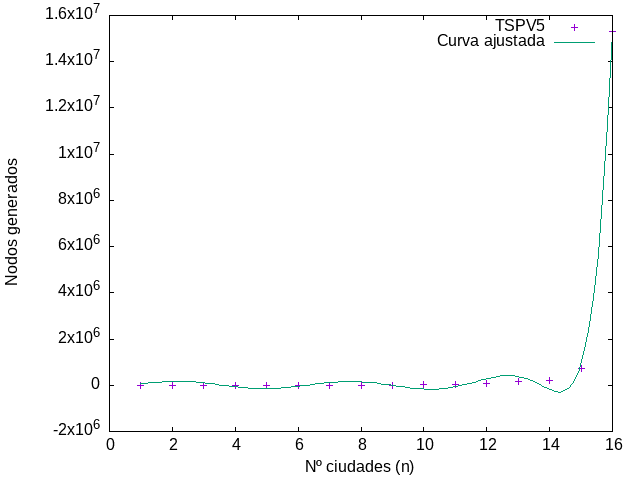
\includegraphics[width=\textwidth]{imagenes/cota1/eficiencia_nodos_bb/CurvaAjustada_n9.png}
        \caption{Polinomio de grado 9}
    \end{subfigure}
    \begin{subfigure}[b]{0.45\textwidth}
        \centering
        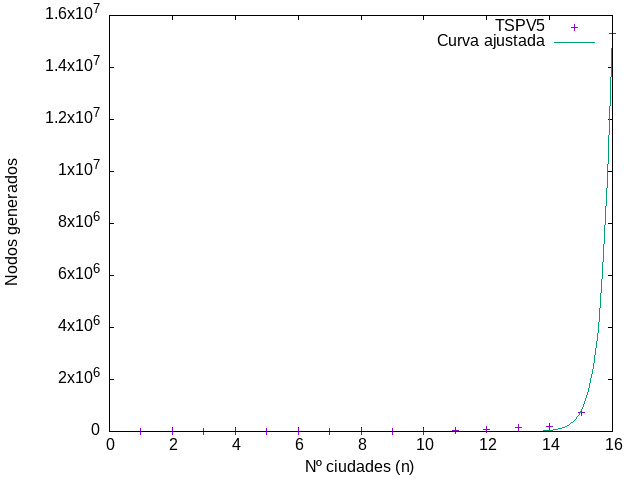
\includegraphics[width=\textwidth]{imagenes/cota1/eficiencia_nodos_bb/CurvaAjustada_exp.png}
        \caption{Exponencial $O(e^{n})$}
    \end{subfigure}
\end{figure}

Podemos observar que ambos ajustes son muy malos. Probemos aumentando el grado del polinomio.

Comparemos sus \textbf{varianzas residuales} para ver cual ajusta mejor a la función:
\begin{itemize}
    \item Exponencial:
    \lstinputlisting[firstline=473, lastline=491,numbers=none]{imagenes/cota1/eficiencia_nodos_bb/fit.log}
    \item Polinomio de grado 9:
    \lstinputlisting[firstline=367, lastline=383,numbers=none]{imagenes/cota1/eficiencia_nodos_bb/fit.log}
\end{itemize}

Podemos ver que la función exponencial ajusta mejor al número de nodos generados en base al tamaño de entrada. En este caso, si nos fijamos en la varianza residual, podemos ver que la de la función exponencial es mucho menor (un orden menos) que la del polinomio. Si tomamos como $p(n) = O(e^{n})$ nos queda:

\begin{equation*}
    O(p(n)(n + \log{p(n)}) + n^{2}) = O(e^{n}(n + \log{e^{n}}) + n^{2})
    = O(n\:e^{n} + e^{n}\log{n^{9}}) = O(n\:e^{n})
\end{equation*}

Por otro lado si escogiésemos el polinomio de grado 9, nos quedaría al final un polinomio de grado 10.

\myparagraph{Eficiencia empírica}

Veamos ahora la eficiencia empírica de nuestro algoritmo branch and bound para la cota 1.

\begin{figure}[H]
    \centering
    \begin{subfigure}[b]{0.45\textwidth}
        \centering
        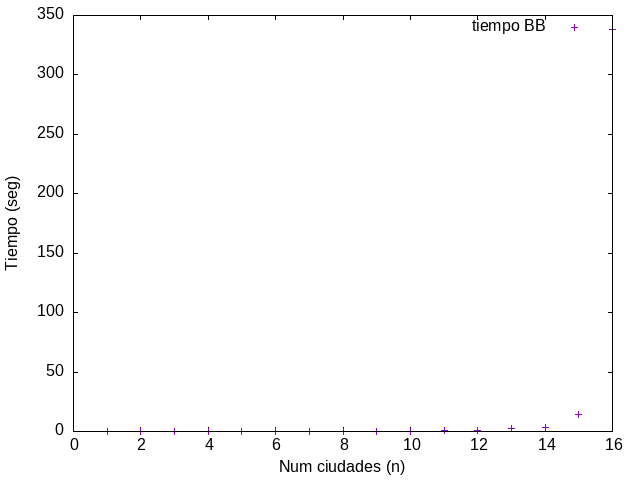
\includegraphics[width=\textwidth]{imagenes/cota1/ef_bb/TSP_BB_empirica_points.png}
        \caption{Puntos}
    \end{subfigure}
    \begin{subfigure}[b]{0.45\textwidth}
        \centering
        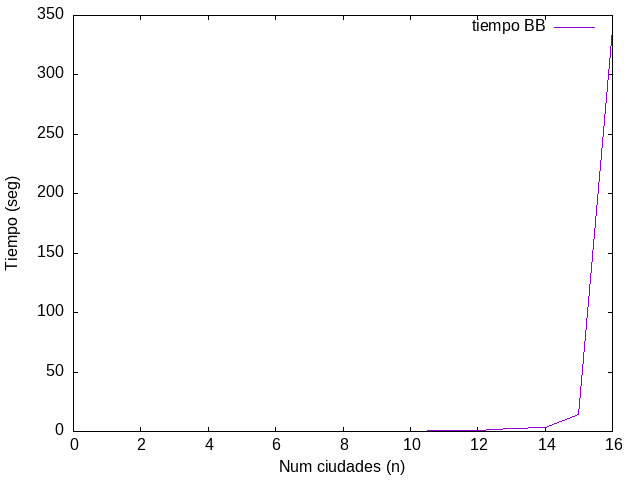
\includegraphics[width=\textwidth]{imagenes/cota1/ef_bb/TSP_BB_empirica_lines.png}
        \caption{Líneas}
    \end{subfigure}
\end{figure}

Podemos ver que la complejidad crece muy rápidamente pero con picos notables carácteristicos de branch and bound. Esto se debe a lo que hablamos antes, que el número de nodos generados no depende exclusivamente del tamaño de entrada, sino que cada caso particular es propenso a tener más o menos podas.
 
\myparagraph{Eficiencia híbrida}

Procedamos ahora a ajustar los datos obtenidos para la eficiencia empírica mediante la expresión obtenida en la eficiencia teórica. En este caso probaremos tanto con el ajuste exponencial $O(n\:e^{n})$ como con el ajuste del polinomio de grado 9 (que nos queda un polinomio de grado 10).

\begin{figure}[H]
    \centering
    \begin{subfigure}[b]{0.45\textwidth}
    \centering
    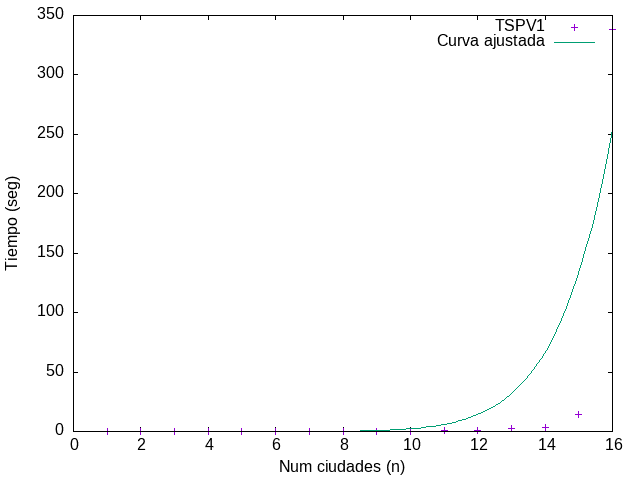
\includegraphics[width=\textwidth]{imagenes/cota1/ef_bb/ef_ajustada.png}
    \caption{Tiempo ajustado por $O(n\:e^{n})$}
    \label{fig:enter-label}
    \end{subfigure}
    \begin{subfigure}[b]{0.45\textwidth}
    \centering
    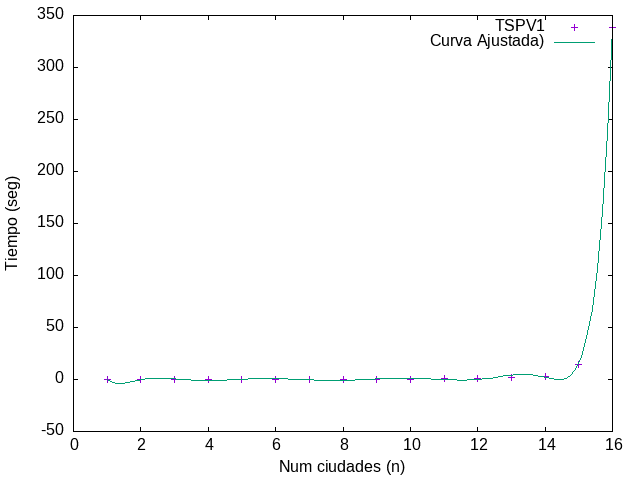
\includegraphics[width=\textwidth]{imagenes/cota1/ef_bb/ef_ajustada_n10.png}
    \caption{Tiempo ajustado por polinomio de grado 10}
    \label{fig:enter-label1}
    \end{subfigure}
\end{figure}

Veamos la varianza residual del ajuste de la figura \ref{fig:enter-label}:
\begin{lstlisting}[numbers=none]
variance of residuals (reduced chisquare) = WSSR/ndf   : 698.618

Final set of parameters            Asymptotic Standard Error
=======================            ==========================
a               = 2.1293e-06       +/- 1.745e-07    (8.196%)
\end{lstlisting}

Veamos la varianza residual del ajuste de la figura \ref{fig:enter-label1}:
\begin{lstlisting}[numbers=none]
variance of residuals (reduced chisquare) = WSSR/ndf   : 2.19275

Final set of parameters            Asymptotic Standard Error
=======================            ==========================
a0              = 179.028          +/- 80.89        (45.18%)
a1              = -460.203         +/- 195.5        (42.48%)
a2              = 463.496          +/- 182.8        (39.43%)
a3              = -246.808         +/- 89.74        (36.36%)
a4              = 78.3653          +/- 26.2         (33.43%)
a5              = -15.7263         +/- 4.831        (30.72%)
a6              = 2.04334          +/- 0.577        (28.24%)
a7              = -0.171328        +/- 0.0445       (25.98%)
a8              = 0.00894024       +/- 0.002138     (23.92%)
a9              = -0.000263844     +/- 5.817e-05    (22.05%)
a10             = 3.36193e-06      +/- 6.839e-07    (20.34%)
\end{lstlisting}

Aquí observamos que aunque en principio la función exponencial aproximaba mejor a la función de número de nodos, podemos ver en el caso de eficiencia, la varianza de la expresión obtenida utilizando el polinomio de grado 9 es menor que el de la exponencial.

Como podemos ver, el ajuste está lejos de ser perfecto, como era de esperarse por no poder ajustar bien el número de nodos generados, pero aproxima medianamente la complejidad temporal de branch and bound para la cota 1, como se puede ver de la varianza residual.

\subsubsection{Funcion cota 2}

\myparagraph{Eficiencia teórica-híbrida}
En primer lugar, la eficiencia de esta función de cota, como ya hemos comentado anteriormente es del orden $O(n^2)$ en el caso peor, es decir, 
$O(q(n)) = O(n^2)$. Por otra parte, calculando el número de nodos generados obtenemos los siguientes datos (hemos trabajado entre 4-17 ciudades debido a las limitaciones HW): 

\begin{figure}[H]
    \centering
    \begin{subfigure}[b]{0.45\textwidth}
        \centering
        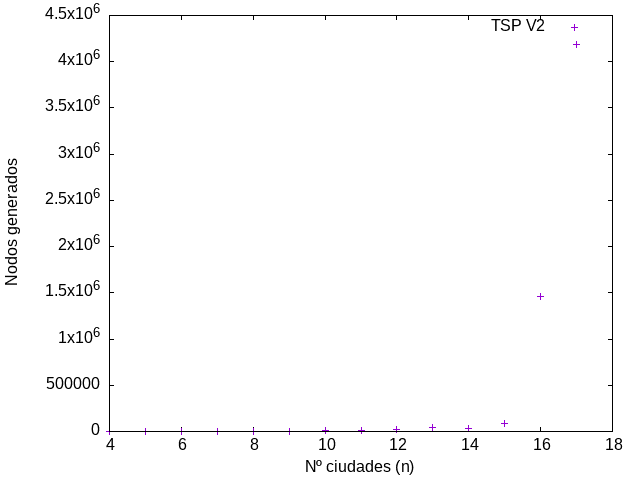
\includegraphics[width=\textwidth]{imagenes/Data/salidaSoloPuntos.png}
        \caption{Puntos.}
    \end{subfigure}
    %\hfill
    \begin{subfigure}[b]{0.45\textwidth}
        \centering
        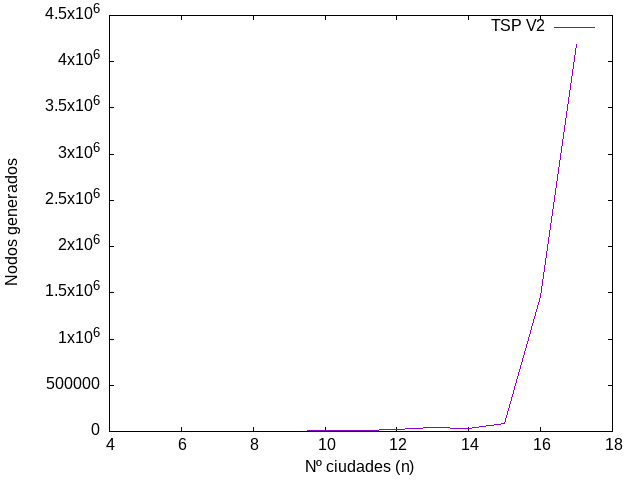
\includegraphics[width=\textwidth]{imagenes/Data/salidaSoloLineas.png}
        \caption{Lineas.}
    \end{subfigure}
\end{figure}

Podemos ver que la velocidad de crecimiento sigue siendo factorial o exponencial. En un intento de aproximarlos por polinomios obtenemos un total fracaso: 

\begin{figure}[H]
    \centering
    \begin{subfigure}[b]{0.45\textwidth}
        \centering
        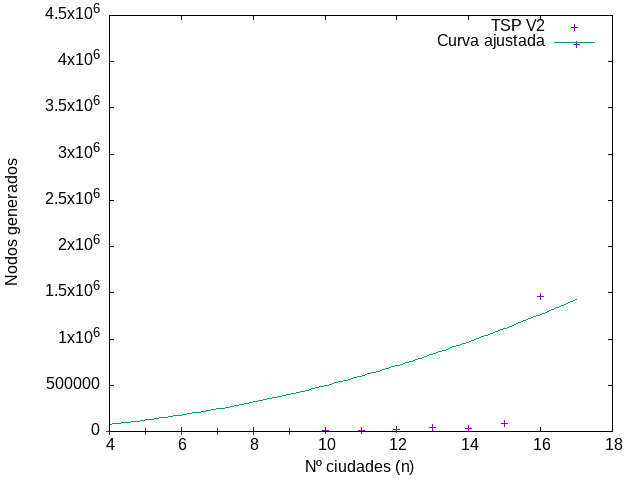
\includegraphics[width=\textwidth]{imagenes/Data/CurvaAjustadaCuadratica.png}
        \caption{Cuadratica.}
    \end{subfigure}
    %\hfill
    \begin{subfigure}[b]{0.45\textwidth}
        \centering
        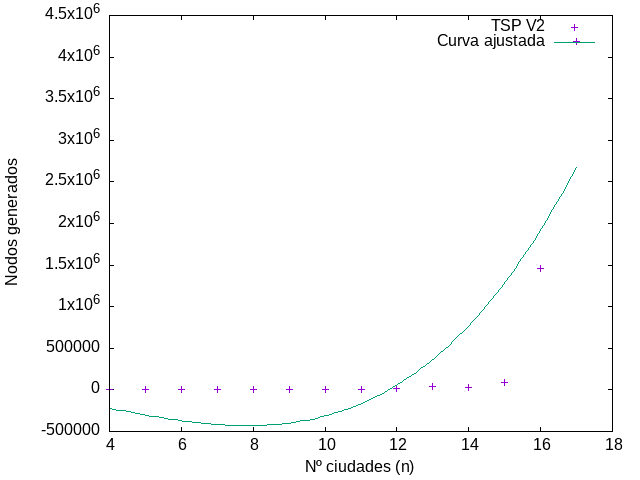
\includegraphics[width=\textwidth]{imagenes/Data/CurvaAjustadaCubica.png}
        \caption{Cubica.}
    \end{subfigure}
\end{figure}

Aproximando mediante funciones exponenciales y factoriales obtenemos 
mejores resultados: 

\begin{figure}[H]
    \centering
    \begin{subfigure}[b]{0.45\textwidth}
        \centering
        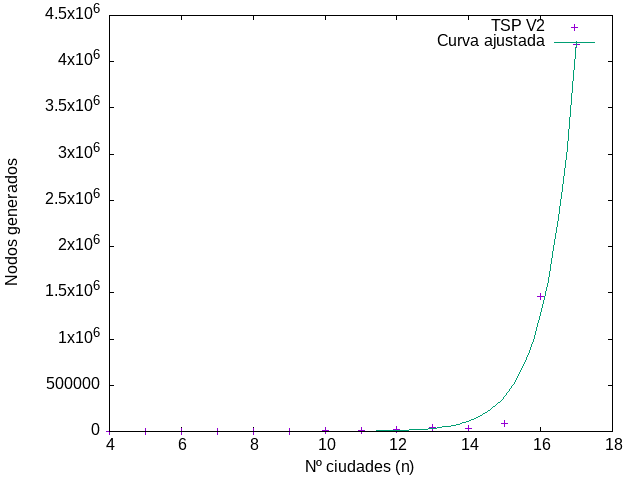
\includegraphics[width=\textwidth]{imagenes/Data/CurvaAjustada.png}
        \caption{Exponencial con $f(x)=0.0054*e^{1.2x}$}
    \end{subfigure}
    %\hfill
    \begin{subfigure}[b]{0.45\textwidth}
        \centering
        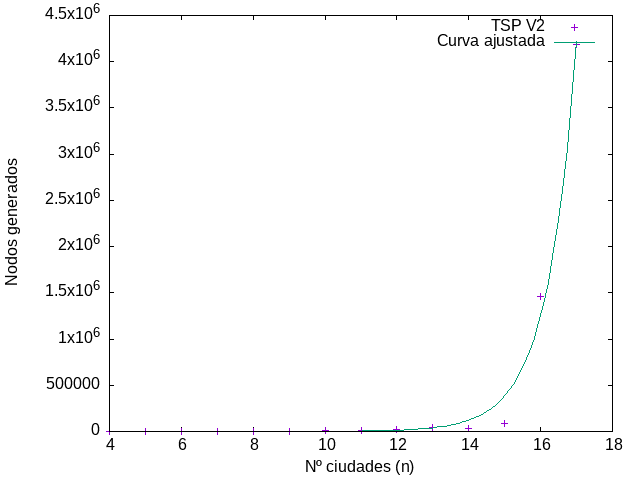
\includegraphics[width=\textwidth]{imagenes/Data/CurvaAjustadaFactorial.png}
        \caption{Exponencial con $f(x)=14.59 \Gamma(0.55(x+1)) $}
    \end{subfigure}
\end{figure}

Graficamente son practicamente idénticas, pero analizando los errores más a fondo tenemos:

\begin{itemize}
    \item Análisis de la regresión facorial: 
    \lstinputlisting[language=C++, firstline=21, lastline=30]{imagenes/fit.log}
    \item Análisis de la regresión exponencial:
    \lstinputlisting[language=C++, firstline=57, lastline=66]{imagenes/fit.log}
\end{itemize}

A la vista de los datos obtenidos, notamos que la diferencia entre ellos con estos datos es también casi irrelevante, así, tomaremos el exponencial por ser levemente menor el error, $O(p(n)) = O(e^x)$. 

A la vista de $O(p(n)) = O(e^x)$ y $O(q(n)) = O(n^2)$ tenemos que la eficiencia de BB con esta función de cota queda de la siguiente manera: 
\[
T(n) = p(n)(n\cdot q(n)+\log{p(n)}) \in O(e^n\cdot(n^3 + \log{e^n})) = O(n^3 e^n)
\]

\myparagraph{Eficiencia empírica e híbrida: }

Ejecutando el programa con diferentes tamaños de entrada (3-17) obtenemos los siguientes datos:

\begin{figure}[H]
    \centering
    \begin{subfigure}[b]{0.45\textwidth}
        \centering
        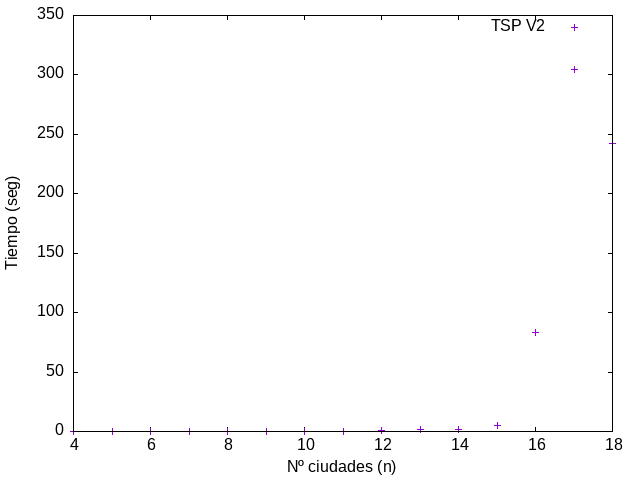
\includegraphics[width=\textwidth]{Sucio_Olga/BB_ajuste2/salidaSoloPuntos.png}
        \caption{Puntos}
    \end{subfigure}
    %\hfill
    \begin{subfigure}[b]{0.45\textwidth}
        \centering
        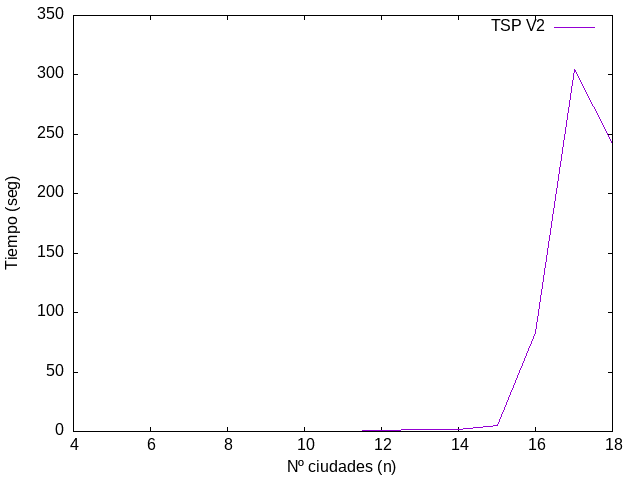
\includegraphics[width=\textwidth]{Sucio_Olga/BB_ajuste2/salidaSoloLineas.png}
        \caption{Lineas}
    \end{subfigure}
\end{figure}

Como era de esperar los tiempos crecen exponencialmente según los datos y además son muy inestables, esto es debido, como ya hemos comentado anteriormente, a que la poda ayuda a reducir el tiempo según el caso pero no determina el comportamiento del algoritmo. 

Ajustándolo con una curva del tipo $f(x)=a x^3 e^{b x}$ obtenemos el siguiente resultado: 
\begin{figure}[H]
    \centering
    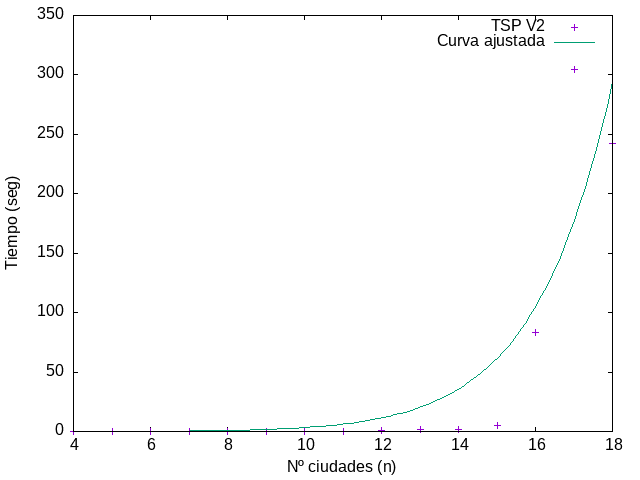
\includegraphics[width=0.45\textwidth]{Sucio_Olga/BB_ajuste2/CurvaAjustadaExponencial.png}
    \caption*{$f(x)=0.0001 x^3 e^{0.339717x}$}
\end{figure}

Veamos la calidad de este ajuste: 
\lstinputlisting[language=C++, firstline=23, lastline=32]{Sucio_Olga/BB_ajuste2/fit.log}

Podemos ver esta regresión tiene una varianza residual del orden $10^3$ y un error asintótico del 230.5\%, lo cual quiere decir que nuestro ajuste no es del todo preciso. En su defensa, la función poda depende mucho del caso a tratar, mejora la eficiencia del algoritmo pero no de manera estable, y por tanto hace incluso más difícil predecir el comportamiento del algoritmo ya que tiene un factor del azar intrínseco.

En conclusión, tenemos una curva que predice el comportamiento  del algoritmo de manera no muy precisa pero ofrece una aproximación de este.
\subsubsection{Funcion cota 3}

A continuación, pasamos a estudiar la eficiencia del algoritmo BranchAndBound al utilizar la función de cota tercera. Nuevamente, deberemos estimar el número de nodos generados por una función y como ya sabemos que nuestra cota es cuadrática en el número de ciudades del problema, la eficiencia será de:

\[
    O(n^3 \cdot num\_nodos)
\]

Al calcular el número de nodos, obtenemos:

\begin{table}[h!]
\centering
\begin{tabular}{|c|c|}
\hline
\textbf{Ciudades} & \textbf{Nodos generados} \\
\hline
1 & 1 \\
\hline
2 & 2 \\
\hline
3 & 5 \\
\hline
4 & 12 \\
\hline
5 & 25 \\
\hline
6 & 55 \\
\hline
7 & 166 \\
\hline
8 & 379 \\
\hline
9 & 570 \\
\hline
10 & 977 \\
\hline
11 & 570 \\
\hline
12 & 428 \\
\hline
13 & 1290 \\
\hline
14 & 1170 \\
\hline
15 & 6398 \\
\hline
16 & 23467 \\
\hline
17 & 243090 \\
\hline
18 & 27657 \\
\hline
19 & 12016 \\
\hline
\end{tabular}
\caption{Nodos generados para la cota 3 por el algoritmo branch \& bound}
\label{tab:datos}
\end{table}

Utilizaremos las mismas regresiones que en la sección \ref{subsubsection:nodes_f_cota3}, para ver, cuál de ellas tiene menor varianza residual:

\begin{figure}[H]
    \centering
    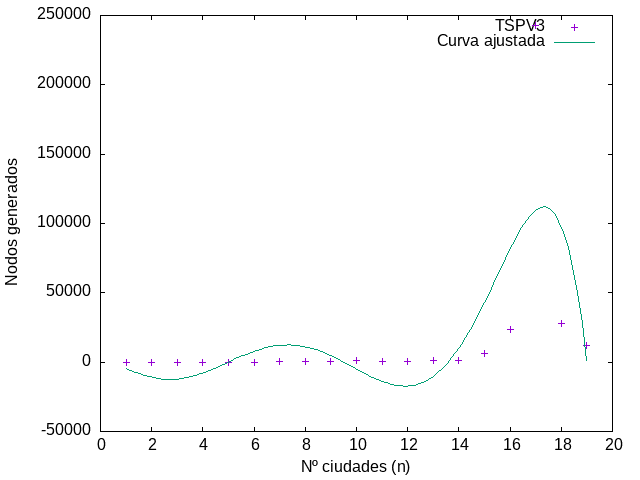
\includegraphics[width=0.7\textwidth]{imagenes/cota3/CurvaAjustada_n6_bb.png}
    \caption*{$f(x)=-0.616606 \cdot x^6 + 29.0489\cdot x^5 -480.284 \cdot x^4 + 3266.63 \cdot x^3 -7569.32 \cdot x^2 + 1.26687 \cdot x + 1.02253$}
\end{figure}

\lstinputlisting[language=C++, firstline=223, lastline=237]{imagenes/cota3/fit_bb.log}

\begin{figure}[H]
    \centering
    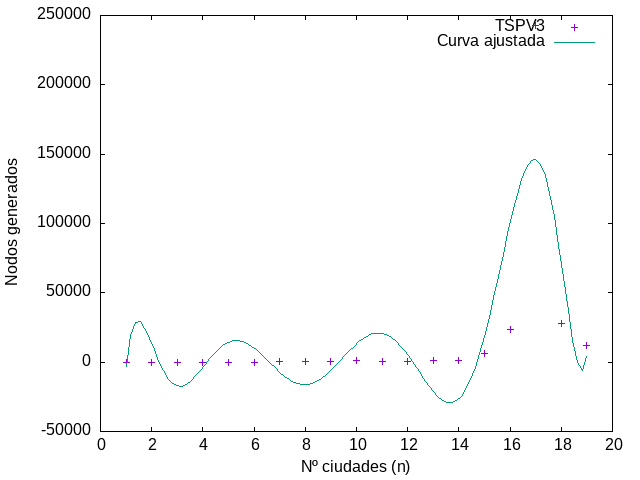
\includegraphics[width=0.7\textwidth]{imagenes/cota3/CurvaAjustada_n9_bb.png}
    \caption*{$f(x)=0.01728 \cdot x^9 -1.51841 \cdot x^8 + 56.1232 \cdot x^7 -1135.67  \cdot x^6 + 13720.9 \cdot x^5 -101300 \cdot x^4 + 449324 \cdot x^3 -112930 \cdot x^2 + 1417440 \cdot x -651607$}
\end{figure}

\lstinputlisting[language=C++, firstline=367, lastline=384]{imagenes/cota3/fit_bb.log}


Nuevamente, las gráficas no aproximan ni por asomo a los puntos, lo cual lo refleja el alto valor de la varianza residual, aunque de todas las regresiones que se han hecho son las dos con varianza residual más baja. Es por eso que nos quedaremos con estas regresiones, en particular con la mejor de ellas: $n^9$. Siguiendo este modelo podríamos decir que nuestro algoritmo branch \& bound con la cota 3 tiene una eficiencia de $O(n^{12})$, aunque esto no tenga ningún sentido. \\

Aún así vamos a ajustar la gráfica de los tiempos por un polinomio de grado 12 y ver qué ocurre:

\lstinputlisting[language=C++, firstline=24, lastline=43]{imagenes/cota3/fittiempos_bb.log}

\begin{figure}[H]
    \centering
    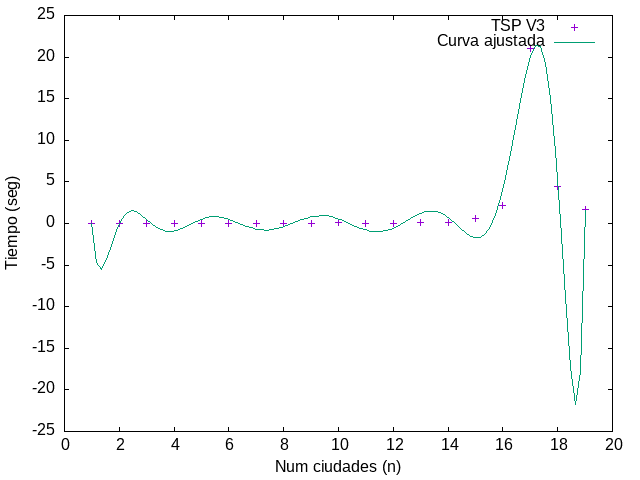
\includegraphics[width=0.7\textwidth]{imagenes/cota3/tiempos_bb.png}
    \caption*{$f(x)=2.07075 \cdot 10^{-8} \cdot x^{12} -2.38616 \cdot 10^{-6} \cdot x^{11} + 0.000121514 \cdot x^{10} -0.00360276  \cdot x^9 + 0.0689667 \cdot x^8 -0.893475  \cdot x^7 +7.9848  \cdot x^6 -49.2475 \cdot x^5 +206.287 \cdot x^4 -566.434  \cdot x^3 +955.524 \cdot x^2 -874.755 \cdot x +321.485$}
\end{figure}

Aunque la varianza residual nos haya salido considerablemente menor, insistimos en que esta forma de modelizar el tiempo en función del número de ciudades no tiene mucho sentido al no seguir el número de nodos una monotonía respecto al número de ciudades.


\newpage
\section{Análisis comparativo del rendimiento}
Vamos a comparar el rendimiento entre las tres funciones de cotas para distintos tamaños de entrada, entre 3 a 15-17-19, según la cota, debido a limitaciones HW. Para ello comenzaremos con la implementación de BB donde compararemos las tres funciones de cotas tanto por el número de nodos generados como por el tiempo de ejecución. 
Seguido, haremos lo mismo con backtraking. Y finalmente comparemos ambas implementaciones.

\subsection{Análisis comparativo con Branch and Bound}

Ejecutando Branch and Bound utilizando las tres funciones de cotas obtenemos los siguientes datos:

%% Hay un lapsus en el nombre de las imágenes, pero son BB 
\begin{figure}[H]
    \centering
    \begin{subfigure}[b]{0.45\textwidth}
        \centering
        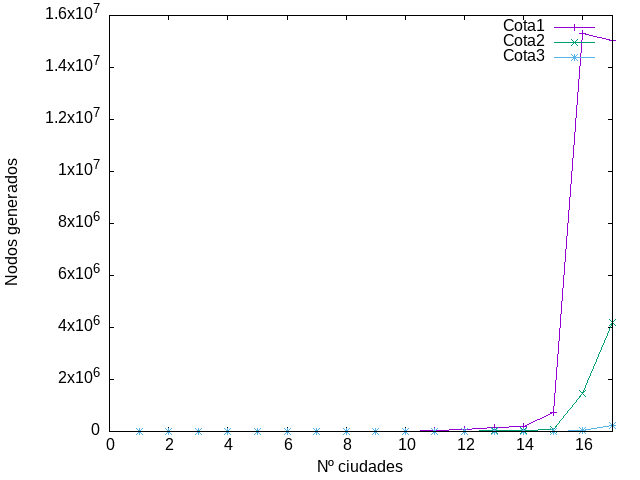
\includegraphics[width=\textwidth]{Sucio_Olga/img/Comparativa_nodos_BB_linespoints.png}
        \caption{Comparativa nodos generados.}
    \end{subfigure}
    %\hfill
    \begin{subfigure}[b]{0.45\textwidth}
        \centering
        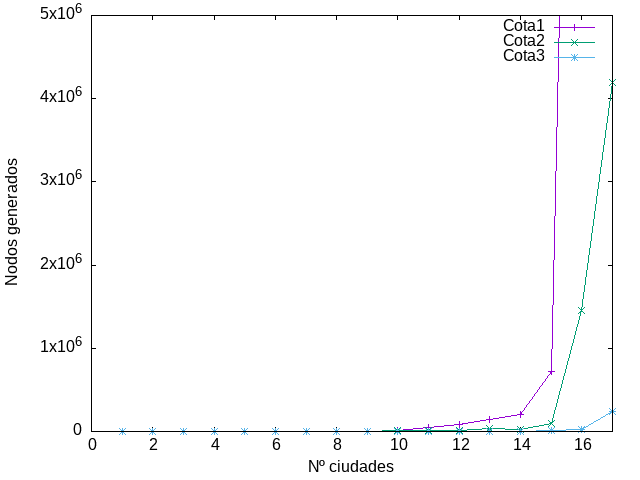
\includegraphics[width=\textwidth]{Sucio_Olga/img/Comparativa_nodos_BB_linespointsAcotado.png}
        \caption{Nodos generados (escala aumentada).}
    \end{subfigure}
\end{figure} 

%% Insertar las gráficas tiempos y explicarlas 
\begin{figure}[H]
    \centering
    \begin{subfigure}[b]{0.45\textwidth}
        \centering
        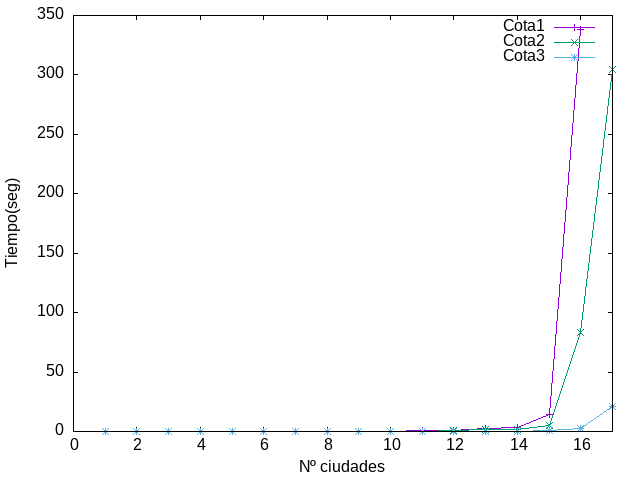
\includegraphics[width=\textwidth]{Sucio_Olga/img/Comparativa_tiempos_BB_linespoints.png}
        \caption{Tiempos de ejecución}
    \end{subfigure}
    %\hfill
    \begin{subfigure}[b]{0.45\textwidth}
        \centering
        \includegraphics[width=\textwidth]{Sucio_Olga/img/Comparativa_tiempos_BB_linespointsAcotado.png}
        \caption{Tiempo de ejución (escala aumentada).}
    \end{subfigure}
\end{figure}

De los datos podemos ver que la función de cota3 es la mejor tanto en número de nodos generados como en tiempo de ejecución, seguido de la cota2.
Por tanto, la mejor cota con la implementación de Branch and Bound es la cota 3. 

\subsection{Análisis comparativo con Backtraking}

Ejecutando backtraking utilizando las tres funciones de cotas obtenemos los siguientes datos: 

\begin{figure}[H]
    \centering
    \begin{subfigure}[b]{0.45\textwidth}
        \centering
        \includegraphics[width=\textwidth]{Sucio_Olga/img/Comparativa_nodos_BK_linespointsAcotado.png}
        \caption{Comparativa nodos generados.}
    \end{subfigure}
    %\hfill
    \begin{subfigure}[b]{0.45\textwidth}
        \centering
        \includegraphics[width=\textwidth]{Sucio_Olga/img/Comparativa_tiempos_BK_linespointsAcotado.png}
        \caption{Tiempo de ejecución.}
    \end{subfigure}
\end{figure} 

%% Insertar gráficas y comentarlas 
Otra vez, vemos que la tercera cota es la más eficiente, tanto en número de nodos generados como en tiempo de ejecución, seguida de la primera cota. Podemos ver que esta vez la cota1 es mejor que la cota2 en tiempo de ejecución, a pesar de no serlo en número de nodos generados. Esto puede ser debido a que la cota2 tenga eficiencia cuadrádica mientras que la cota 1 tiene eficiencia constante. Notemos que el hecho de que la cota2 sea mejor que la cota1 en BB tiene sentido puesto que en este se puede elegir los caminos a seguir según la cota y aquí en BK está limitado a seguir el camino sistemático, es decir la cota solo puede influir en la poda pero no en la elección. \\  

Por tanto, la mejor cota con la implementación de backtraking es la cota 3. 

\myparagraph{Comparación entre Branch and Bound y Backtraking} 

Aquí vamos a comparar todos los resultados: 

\begin{figure}[H]
    \centering
    \begin{subfigure}[b]{0.45\textwidth}
        \centering
        \includegraphics[width=\textwidth]{Sucio_Olga/img/Comparativa_nodos_linespoints.png}
        \caption{Nodos generados}
    \end{subfigure}
    %\hfill
    \begin{subfigure}[b]{0.45\textwidth}
        \centering %%Falta tiempo
        \includegraphics[width=\textwidth]{Sucio_Olga/img/Comparativa_nodos_linespointsAcotado.png}
        \caption{Nodos generados (escala aumentada)}
    \end{subfigure}
\end{figure}

\begin{figure}[H]
    \centering
    \begin{subfigure}[b]{0.45\textwidth}
        \centering
        \includegraphics[width=\textwidth]{Sucio_Olga/Comparativa_tiempos_linespoints.png}
        \caption{Tiempo de ejecución.}
    \end{subfigure}
    %\hfill
    \begin{subfigure}[b]{0.45\textwidth}
        \centering %%Falta tiempo
        \includegraphics[width=\textwidth]{Sucio_Olga/Comparativa_tiempos_linespointsAcotado.png}
        \caption{Tiempo de ejecución (escala aumentada).}
    \end{subfigure}
\end{figure}

Vemos claramente que las versiones de BB son generalmente más eficientes en tiempo de ejecución que las de BK, excepto en la cota1 que concuerda con lo que explicamos anteriormente. Por otra parte, es claro que la cota 3, ya sea en versión BB o en versión BK, genera menos nodos y tarda menos que cualquier otra función de cota. Veamos ahora más a fondo la función de cota 3: 

\begin{figure}[H]
    \centering
    \begin{subfigure}[b]{0.45\textwidth}
        \centering
        \includegraphics[width=\textwidth]{Sucio_Olga/img/Comparativa_nodes3_linespoints.png}
        \caption{Nodos generados}
    \end{subfigure}
    %\hfill
    \begin{subfigure}[b]{0.45\textwidth}
        \centering %%Falta tiempo
        \includegraphics[width=\textwidth]{Sucio_Olga/img/Comparativa_tiempos_3_linespoints.png}
        \caption{Tiempo de ejecución.}
    \end{subfigure}
\end{figure}

Vemos que el número de nodos generados en ambos casos es parecido y BB en tiempo de ejecución es ligeramente más rápido, en especial cuanto mas aumenta el tamaño (tal y como se explica en la definición del mismo) con lo cual podemos concluir que BB aunque tenga más exigencias de memoria y en principio su eficiencia en el caso peor sea peor que la de branch and bound (debido a la \verb|priority_queue|) encuentra la solución óptima antes generalmente.

\myparagraph{Conclusión de la comparativa}

Vemos claramente que en todas las comparativas se mantiene en la mayoría de los casos una correlación entre al número de nodos generados y el tiempo de ejecución, la cota que menos nodos genera suele resultar también en ser la más eficiente. Notemos que aunque se realicen más cómputo por nodo, empeorando así la eficiencia teórica, para podar más ramas, puede resultar rentable (en comparación con un número inicial de nodos del orden factorial). Esto se refleja en el hecho de que la cota1 aun siendo del orden $O(1)$ y la cota 3 del orden $O(n^2)$, esta última, que es la que menos nodos genera, es la mejor y la primera, que la que más nodos genera, es la peor. El caso de la cota1 y cota2 es un caso particular. 

Cabe mencionar también el comportamiento irregular que obtenemos en el número de nodos generados y en el tiempo de ejecución según la instancia, esto, como mencionamos anteriormente, es porque hay un factor del azar intrínseco en nuestro algoritmo. Podemos perfectamente encontrar la solución buscada en la primera rama que recorramos como encontrarla en la última rama. Así, no nos debe extrañar los picos de las gráficas, eso sí, sí que podemos ver que todos siguen un comportamiento esencialmente creciente. 

\newpage
\section{Conclusiones}
En el transcurso de esta práctica, hemos logrado una comprensión profunda y una implementación eficaz de técnicas algorítmicas avanzadas, específicamente Backtracking y Branch and Bound, aplicadas a la resolución del problema del viajante de comercio. Esta experiencia ha complementado y extendido nuestros conocimientos teóricos, permitiéndonos enfrentar y superar retos complejos mediante la exploración sistemática de grafos.

La práctica nos ha permitido no solo diseñar e implementar algoritmos utilizando estas técnicas, sino también realizar un análisis detallado de su eficiencia. Hemos evaluado la eficacia de diversas funciones de cota, observando cómo impactan en el rendimiento de los algoritmos en términos de tiempo de ejecución y número de nodos generados. Este análisis comparativo ha sido crucial para entender las fortalezas y debilidades de cada enfoque en diferentes escenarios, reforzando la importancia de una correcta selección y validación de las funciones de cota.

Durante el desarrollo de la práctica, se han manifestado conceptos teóricos clave en la implementación y optimización de los algoritmos, tales como:

\begin{itemize}
\item La importancia de diseñar funciones de cota efectivas que mejoren significativamente la eficiencia de los algoritmos de Backtracking y Branch and Bound.
\item La observación de que, aunque las diferencias en hardware y software pueden afectar los tiempos de ejecución absolutos, la eficiencia relativa entre diferentes algoritmos y enfoques permanece consistente, resaltando la robustez de nuestras comparaciones.
\end{itemize}

Además de los aspectos técnicos, la práctica ha fomentado el desarrollo de habilidades blandas esenciales. El trabajo en equipo ha sido fundamental, promoviendo la colaboración, el intercambio de ideas y la distribución equitativa de tareas. Estas competencias transversales, junto con el pensamiento crítico y la comunicación efectiva, han enriquecido nuestra experiencia, preparándonos mejor para futuros desafíos tanto en el ámbito académico como profesional.

Finalmente, la documentación exhaustiva de nuestro trabajo, que incluye el diseño, implementación y análisis de los algoritmos, ha sido un ejercicio valioso en comunicación técnica. Esta memoria no solo facilita la evaluación por parte de los profesores, sino que también sirve como un recurso de referencia para futuros proyectos.

En resumen, esta práctica ha sido una oportunidad invaluable para aplicar y profundizar en técnicas algorítmicas avanzadas, desarrollar habilidades analíticas y colaborativas, y reforzar nuestra preparación para enfrentar problemas complejos en el campo de la ciencia de la computación. Consideramos que esta experiencia ha sido altamente enriquecedora, proporcionando herramientas y perspectivas cruciales para nuestro desarrollo académico y profesional.


\end{document}

